\documentclass[a4paper, 11pt]{article}
 


%%%%%%%%%%%%%%%%%%%%%%%%%%%%%%%%%
%	 PACKAGES	%
%%%%%%%%%%%%%%%%%%%%%%%%%%%%%%%%%
% Codierung von in und Output
\usepackage[utf8]{inputenc}
\usepackage[T1]{fontenc}

% AMS-Pakete für Mathe
\usepackage{amsthm,amssymb,amsmath}

% Sprachpaket neue rechtschreibung
\usepackage[ngerman]{babel} 


\usepackage[many]{tcolorbox}
\usepackage[dvipsnames]{xcolor}


%Header und Seitengrösse
\usepackage{fancyhdr}
\usepackage{geometry}

% Paket für Links im PDF (glaubs)!
\usepackage[hidelinks]{hyperref}

%Paket um ganze pdf-File zu importieren (Arbeitsblätter aus Analysis DMK)
\usepackage{pdfpages}

%TColorbox nutzt Theoreme und bessere Verweise
\tcbuselibrary{theorems}
\usepackage{cleveref}

%Package, um Aufgaben auf mehrere Spalten zu verteilen.
\usepackage{tasks}

% Programmcode-Darstellung
% \usepackage{listings}
% \lstset{basicstyle=\ttfamily}
% \makeatletter
% \def\BState{\State\hskip-\ALG@thistlm}
% \makeatother
\usepackage{listings}
% \usepackage{xcolor}
\lstset{basicstyle=\ttfamily, language= Python}
\definecolor{codekeyword}{rgb}{0.11,0.53,0.63}
\definecolor{codenumbers}{rgb}{0.71,0.21,0.30}
\definecolor{codeoperation}{rgb}{0.57,0.32,0.59}
\definecolor{codecomment}{rgb}{0.17,0.59,0.28}
\definecolor{backcolour}{rgb}{0.98,0.97,0.99}
\definecolor{codestring}{rgb}{0.84,0.56,0.16}
\lstdefinestyle{mystyle}{
    backgroundcolor=\color{backcolour},   
    commentstyle=\color{codecomment},
    keywordstyle=\color{codekeyword},
    numberstyle=\tiny\color{black},
    stringstyle=\color{codestring},
    basicstyle=\ttfamily\footnotesize,
    breakatwhitespace=false,         
    breaklines=true,                 
    captionpos=b,                    
    keepspaces=true,                 
    numbers=left,                    
    numbersep=5pt,                  
    showspaces=false,                
    showstringspaces=false,
    showtabs=false,                  
    tabsize=4
}

\lstset{style=mystyle}


\usepackage{graphicx}
\usepackage{hyperref}
\usepackage{array}
\hypersetup{colorlinks=true}

% damit kann man nummerierte Liste unterbrechen und wieder aufnehmen
\usepackage{enumitem} 

%Für mehrere Spalten in Aufgaben
\usepackage{multicol}
	\setlength\multicolsep{5pt}

%%%CHANGE LABEL FIGURE
\usepackage[figurename=Abbildung.]{caption}
\usepackage{subcaption}

%%%%%%%%%%%%%%%%%%%%%%%%%%%%%%%%
%%%%%%%%%%%	LAYOUT	%%%%%%%%%%%%
%%%%%%%%%%%%%%%%%%%%%%%%%%%%%%%%

\geometry{
	a4paper,
	total={165mm,225mm},
	left=25mm,
	top=35mm,
}

%keine Einrückung bei Absatz dafür Abstand
\setlength\parindent{0pt}
\setlength{\parskip}{1em}

%Header
\pagestyle{fancy}
\setlength{\headheight}{13.6pt}
\renewcommand{\sectionmark}[1]{ \markright{#1}{} }
\lhead[L]{M. Anderegg}
\chead{}
\rhead{Komplexe Zahlen - \rightmark}
\lfoot{}
\cfoot{\thepage}
\rfoot{}





%%%%%%%%%%%%%%%%%%%%%%%%%%%%%%%%
%%%%%%%%% TCB-Commands %%%%%%%%%
%%%%%%%%%%%%%%%%%%%%%%%%%%%%%%%%

\newtcbtheorem
[auto counter, number within=section, crefname={beispiel}{beispiele}, Crefname={Beispiel}{Beispiele}] % Nummerierung und Name bei Verweis
{bsp} % Name der Umgebung \begin{bsp}
{Beispiel} %Name der im Titel angezeigt wird
{breakable, enhanced, fonttitle=\bfseries, coltitle = black, colbacktitle = orange!15, righthand width=3cm,
	sharp corners,boxrule=.4pt,colback=orange!5} %%Optionen für die Box. 
	%Breakable und Enhanced lassen zu, dass sich die Box auf zwei Seiten verteilt.
{bsp} %So wird intern auf die Referenz verwiesen.

\newtcbtheorem[auto counter,  crefname={lernaufgabe}{lernaufgaben},
Crefname={Lernaufgabe}{Lernaufgaben}]{LA}{Lernaufgabe}{
	breakable, enhanced, fonttitle=\bfseries, coltitle = black, colbacktitle = cyan!15, righthand width=3cm,
	sharp corners,boxrule=.4pt,colback=white}{LA}

\newtcbtheorem[auto counter, number within=section, Crefname={Übung}{Übungen}]{ueb}{Übung}{
	breakable, fonttitle=\bfseries, coltitle = black, colbacktitle = blue!15, righthand width=3cm,
	sharp corners,boxrule=.4pt,colback=blue!5}{uebng}


\newtcbtheorem[auto counter, number within=section, crefname={definition}{definitionen},
Crefname={Definition}{Definitionen}]{definition}{Definition}{
	breakable, colframe=green!70!black, fonttitle=\bfseries, coltitle = white, colbacktitle = green!70!black, enhanced, attach boxed title to top left={yshift=-0.1in, xshift=0.15in},}{def}

\newtcbtheorem[auto counter, number within=section, crefname={Satz}{Sätze},
Crefname={Satz}{Sätze}]{satz}{Satz}{%
	breakable, lower separated=false,
	colframe=red!70!white, fonttitle=\bfseries, coltitle = white, colbacktitle = red!70!white, enhanced, attach boxed title to top left={yshift=-0.1in,xshift=0.15in},
}{satz}




%%%%%%%%%%%%%%%%%%%%%%
%%%% Mathe-Befehle %%%
%%%%%%%%%%%%%%%%%%%%%%


\newcommand{\N}{\mathbb{N}}
\newcommand{\Z}{\mathbb{Z}}
\newcommand{\Q}{\mathbb{Q}}
\newcommand{\R}{\mathbb{R}}
\newcommand{\C}{\mathbb{C}}
\newcommand{\LL}{\mathbb{L}}
\newcommand{\DD}{\mathbb{D}}
\newcommand{\Ra}{\Rightarrow}

% Komplexe Zahlen
\newcommand{\RE}{\mathrm{Re}}
\newcommand{\IM}{\mathrm{Im}}
\newcommand{\cis}{\mathrm{cis}}


% TikZ
\usepackage{pgfplots}	
\pgfplotsset{compat=1.8}
\usepackage{pgf,tikz}
\usepackage{mathrsfs}
\usetikzlibrary{arrows}


\usetikzlibrary{arrows,positioning,shapes,fit,calc}

\pgfdeclarelayer{background}
\pgfsetlayers{background,main}


\usepackage{subcaption}




\begin{document}

\title{Komplexe Zahlen}
\author{M. Anderegg}
\date{} % sonst wird das Datum im Titel angezeigt
\maketitle 

Während Ihrer Schulzeit haben Sie bereits mehrfach erlebt, wie der Zahlenbereich schrittweise erweitert wurde:
\begin{itemize}
	\item In der Grundschule haben Sie zunächst die natürlichen Zahlen $\N$ kennengelernt, die für das Zählen und einfache Rechenoperationen genutzt werden.
	$$\N=\left\{\hspace{5cm}\right\}$$
    Die Zahlen in dieser Menge kann man unbesorgt addieren und multiplizieren. Beim Subtrahieren kann es aber vorkommen, dass das Resultat ausserhalb den Menge $\N$ liegt. %Zum Beispiel, wenn man $5-7$ rechnet.
  \item Darum wurde dieser Zahlenbereich zu den ganzen Zahlen $\Z$ erweitert, sodass Subtraktionen uneingeschränkt möglich wurden.
		$$\Z=\left\{\hspace{5cm}\right\}$$
    Allerdings kann es sein, dass man bei der Division von zwei ganzen Zahlen ein Resultat erhält, das nicht zur Menge $\Z$ gehört. 
	\item Die nächste Erweiterung führte von den ganzen Zahlen $\Z$ zu den rationalen Zahlen $\Q$, womit Divisionen (ausser durch $0$) durchgeführt werden können.
		$$\Q=\left\{\hspace{5cm}\right\}$$

  \item Schliesslich ermöglichte der Übergang von $\Q$ zu den reellen Zahlen $\R$, auch Lösungen für bestimmte Potenzgleichungen wie $x^2=2$ zu finden oder Konstanten wie $\pi$ zur Beschreibung der Fläche des Einheitskreises anzugeben.
		\end{itemize}

Insgesamt wurde der Zahlenbereich also bereits dreimal erweitert.


$$\textcolor{ForestGreen}{\N}\subset\textcolor{Brown}{\Z}\subset\textcolor{BrickRed}{\Q}\subset\textcolor{RoyalBlue}{\R}$$


\begin{center}
    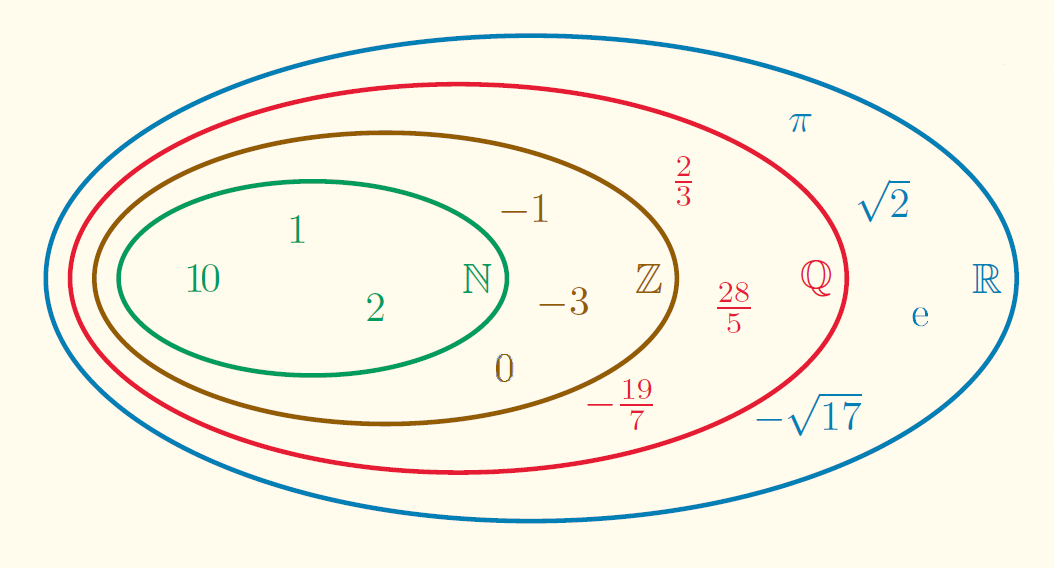
\includegraphics[width = 0.5 \textwidth]{media/zahlenmengen2.png}
\end{center}


Bei all diesen Erweiterungen wurden stets drei wesentliche Punkte eingehalten (\textit{Permanenzprinzip}):

\begin{enumerate}
\item Die alten Zahlenmengen sind stets in den neuen Zahlenmengen enthalten.
\item Alle Rechenoperationen, die mit den alten Zahlen möglich waren, bleiben auch in den neuen Zahlen möglich.
\item Die Rechenregeln der alten Zahlen gelten unverändert auch für die neuen Zahlen.
\end{enumerate}

Da es in $\R$ einfache Gleichungen gibt, wie etwa $x^2 = -1$, die sich zwar formulieren, aber nicht lösen lassen, liegt es nahe, $\R$ zu erweitern. Wie diese Erweiterung unter Einhaltung des Permanenzprinzips durchgeführt werden kann, werden wir im weiteren Verlauf dieser Skripts untersuchen. Das Ergebnis dieser Erweiterung wird die Menge $\C$ der komplexen Zahlen sein, in der insbesondere die Potenzgleichung $x^2 = -1$ eine Lösung besitzt – nämlich die sogenannte imaginäre Einheit $i$.

\clearpage
\section{Die Normalform komplexer Zahlen}
\subsection{Die imaginäre Einheit \texorpdfstring{$i$}{i}}

%Der Ausgangspunkt, um die reellen Zahlen zu den komplexen Zahlen zu erweitern, ist die Gleichung $x^2 = -1$, die in $\R$ aufgestellt, aber nicht gelöst werden kann (das Quadrat einer reellen Zahl ungleich null ist stets positiv). 

\begin{definition}{Die imaginäre Einheit $i$}{}
Die \textit{imaginäre Einheit} $i$ ist eine Zahl, welche die Gleichung $x^2=-1$ erfüllt. Es gilt also: 
$$i^2=-1$$
\end{definition}

Bisher wissen wir nur, dass $i$ keine reelle Zahl ist, da das Quadrat einer reellen Zahl nicht negativ sein kann. Was genau wir uns unter $i$ vorstellen sollten, ist noch nicht ganz klar. Dennoch können wir bereits mit $i$ rechnen, da gemäss dem dritten Punkt des Permanenzprinzips die Rechenregeln aus $\mathbb{R}$ auch für die komplexen Zahlen weiterhin gültig bleiben:



\begin{satz}{Rechnen mit $i$}{}
    \begin{itemize}
        \item Mit der imaginären Einheit $i$ wird gerechnet wie mit einer Variablen.
        \item Alle zweiten und höheren Potenzen von $i$ werden mit Hilfe der Relation $i^2 = -1$ ersetzt.
    \end{itemize}
    \end{satz}

    \begin{bsp}{Rechnen mit $i$}{}
        $i \cdot (3 - (5-3i)) = $

        \vspace*{1cm}

        $i^3 = $
        %\vspace*{1cm}
    \end{bsp}

    \begin{bsp}
    {Neu lösbare Gleichung}{}
    Die Gleichung $x^2 = -4$ ist in der Grundmenge der reellen Zahlen nicht lösbar. Lässt man imaginäre Ergebnisse zu, hat die Gleichung jedoch zwei Lösungen:

    \vspace*{2cm}


    \end{bsp}

    \emph{Bemerkung:}
Man sollte $i$ nicht einfach als $\sqrt{-1}$ schreiben, weil dies in den reellen Zahlen nicht definiert ist. Wenn man mit diesem Wurzelsymbol so rechnet, wie man das aus dem Reellen gewöhnt ist, dann stösst man schnell auf Widersprüche.\footnote{Früheren Mathematikern war die Zahl $i$ übrigens etwas unheimlich. GOTTFRIED WILHELM LEIBNIZ (1646-1716) beispielsweise nannte sie „ein Amphibium zwischen Sein und Nichtsein“, für LEONHARD EULER (1707-1783) war sie eine „unmögliche Zahl“, und noch KARL FRIEDRICH GAUSS (1777-1855) bezeichnete sie im neunzehnten Jahrhundert als „Schatten von Schatten“. Da $i$ also eine „unmögliche Zahl“ war, das heisst keine reelle Zahl, nannte man sie „imaginär" (von lateinisch imaginarius $=$ eingebildet). Die Bezeichnung geht auf RENÉ DESCARTES (1596-1650) zurück.}
$$1=\sqrt{1}=\sqrt{(-1)\cdot(-1)}=\sqrt{-1}\cdot \sqrt{-1}=i\cdot i=-1$$


\begin{ueb}{Erstes Rechnen mit der imaginären Einheit}{uebungzui}
    \begin{enumerate}
        \item Berechnen Sie die Potenzen von $i$:

\begin{enumerate}
	\item $i^2=$
	\item $i^3=$
	\item $i^4=$
	\item $i^5=$
	\item $i^6=$
	\item $i^7=$
	\item $i^{123}=$
\end{enumerate}


\textbf{Beobachtung:} %Die Potenzen von $i$ wiederholen sich in einem Zyklus von vier.

\item Berechnen Sie die folgenden Ausdrücke.

\begin{enumerate}
    \item $i^7 + i^9 + i^{12} + i^4$
    \item $i(-i) + (-i)^2 + i^4 - i^3 - (-i)^4$
    \item $\frac{i^{12} \cdot i^{10} \cdot i^{20}}{i^{44}}$
    \item $(2i - i^3)^2 + (i + 3i^2)^2$
\end{enumerate}
\item Lösen Sie die folgenden quadratischen Gleichungen.

\begin{enumerate}
    \item $x^2 = -9$
    \item $x^2 = -15$
    \item $x^2 + 2x + 2 = 0$
\end{enumerate}
\end{enumerate}
\end{ueb}


\clearpage
\emph{Lösungen}
\begin{enumerate}
\item Berechnen Sie die Potenzen von $i$:
    \begin{enumerate}
        \item $i^2= -1$
        \item $i^3= -i$
        \item $i^4= 1$
        \item $i^5= i$
        \item $i^6= -1$
        \item $i^7= -i$
        \item $i^{123}= -i$
    \end{enumerate}
    
    \item Berechnen Sie die folgenden Ausdrücke:
    \begin{enumerate}
        \item $i^7 + i^9 + i^{12} + i^4 = -i +i +1 +1 = 2$
        \item $i(-i) + (-i)^2 + i^4 - i^3 - (-i)^4 = 1 + (-1) + 1 + i -1 = i$
        \item $\frac{i^{12} \cdot i^{10} \cdot i^{20}}{i^{44}} = -1$
        \item $(2i - i^3)^2 + (i + 3i^2)^2 = -1-6i$
    \end{enumerate}
    
    \item Lösen Sie die folgenden quadratischen Gleichungen:
    \begin{enumerate}
        \item $x^2 = -9 \Rightarrow x = \pm 3i$
        \item $x^2 = -15 \Rightarrow x = \pm \sqrt{15}i$
        \item $x^2 + 2x + 2 = 0 \Rightarrow x = -1 \pm i$
    \end{enumerate}
\end{enumerate}
















\clearpage
\subsection{Die Normalform}
Alle Ergebnisse der \Cref{uebng:uebungzui} sind Zahlen der Form $a+b\cdot i$ mit $a,\ b\in \R$. Letztere bilden die Menge der komplexen Zahlen:

\begin{definition}{Normalform einer komplexen Zahl}{}
\emph{Komplexe Zahlen} sind Zahlen der Form $z=a+b\cdot i$, wobei $a,\ b\in \R$ sind. 

Die Menge der komplexen Zahlen ist: 
$$\C=\left\{a+bi \, | \, a,\ b\in \R\right\}$$

Die reelle Zahlen $a$ bzw. $b$ nennt man \emph{Realteil} bzw.  \emph{Imaginärteil} der komplexen Zahl $z=a+bi$:

$$\RE(a+bi)=a \hspace{4cm} \IM(a+bi)=b$$

Eine Zahl, deren Realteil $0$ ist, nennt man \emph{rein imaginär}.


\end{definition}

\begin{bsp}
{}{}
Bei der Zahl $z = 3-9i$ handelt es sich um eine komplexe Zahl mit
$$\RE(z)=3 \hspace{4cm} \IM(z)=-9$$

\end{bsp}

\begin{itemize}
	\item Das Wort „komplex“ steht hier für „zusammengesetzt“ (Latein complexus = verflochten), da alle komplexe Zahlen aus einem reellen Anteil und einem imaginären Anteil zusammengesetzt sind.
	\item Jede reelle Zahl ist auch eine komplexe Zahl (mit Imaginärteil $0$). Beispiel $-42=-42+0i$.\\	Die Menge $\R$ ist also eine Teilmenge der Menge $\C$:
	$$\textcolor{ForestGreen}{\N}\subset\textcolor{Brown}{\Z}\subset\textcolor{BrickRed}{\Q}\subset\textcolor{RoyalBlue}{\R}\subset\textcolor{DarkOrchid}{\C}$$
\end{itemize}


\begin{center}
    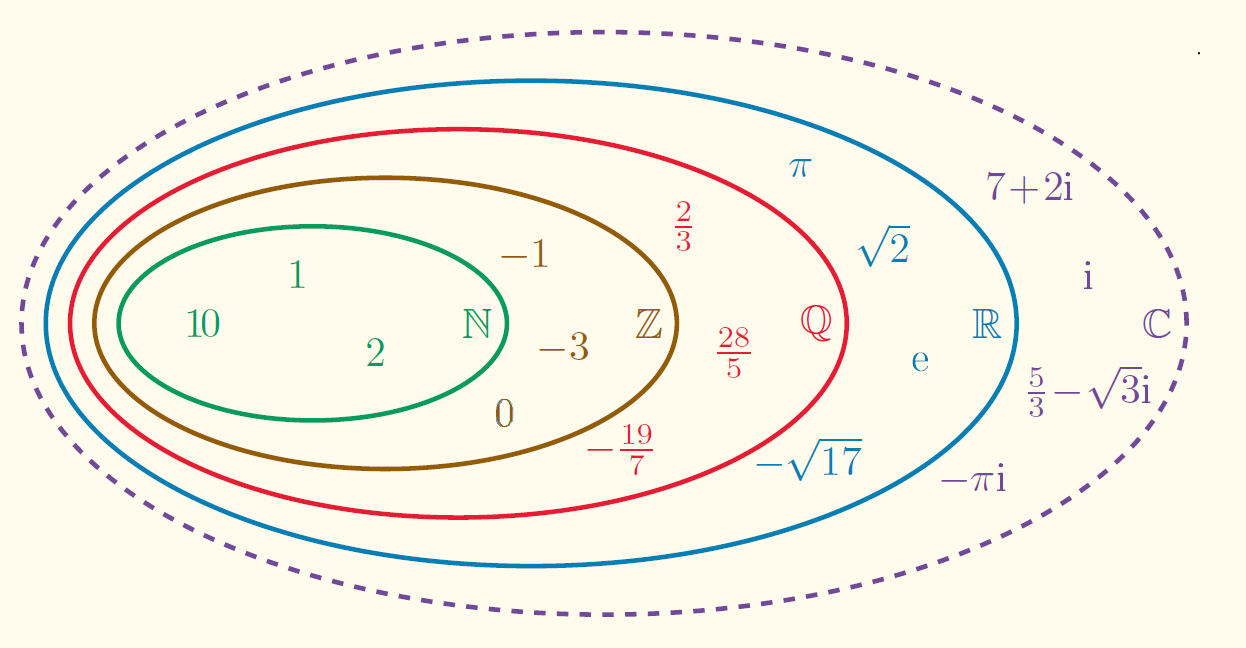
\includegraphics[width = 0.75 \textwidth]{media/zahlenmengen.png}
\end{center}

Bei den beiden Lösungen $x_1 = -1 + i$ und $x_2 = -1 - i$ der Gleichung $x^2 + 2x + 2 = 0$ (Siehe \Cref{uebng:uebungzui}) fällt auf, dass sie sich nur durch im Vorzeichen des Imaginärteils unterscheiden. Solche Zahlen werden konjugiert komplexe Zahlen genannt.

\begin{definition}
    {Die konjugiert komplexe Zahl}{}
    Die zu $z = a + bi$ konjugiert komplexe Zahl $\bar{z}$ ist definiert als 
    $$\bar{z} = a - bi$$

\end{definition}

\begin{ueb}
    {Übungen zur Normalform}{uebZuNormalform}
    \begin{enumerate}
        \item Geben Sie Realteil und Imaginärteil der folgenden komplexen Zahlen an
    
        \begin{enumerate}
            \item $z=-1+4 i$ \hfill $\RE(z)=\phantom{aaaa}$ \hspace{2.5cm} $\IM(z)=\phantom{aaaa}$\hspace{3cm}\phantom{a}
            \item $z=2-5 i$ \hfill $\RE(z)=\phantom{aaaa}$ \hspace{2.5cm} $\IM(z)=\phantom{aaaa}$\hspace{3cm}\phantom{a}
        
            \item $z=-\frac{1}{6}$\hfill $\RE(z)=\phantom{aaaa}$ \hspace{2.5cm} $\IM(z)=\phantom{aaaa}$\hspace{3cm}\phantom{a}
            \item $z=i-\pi$\hfill $\RE(z)=\phantom{aaaa}$ \hspace{2.5cm} $\IM(z)=\phantom{aaaa}$\hspace{3cm}\phantom{a}
        
        \end{enumerate}
        \item Sind die folgenden Aussagen richtig oder falsch? Begründen Sie Ihre Antworten.
        \begin{itemize}
            \item Für alle komplexen Zahlen $z$ gilt: $z=\RE(z)+\IM(z)$.
            \item Für alle komplexe Zahlen $z$ mit $\RE(\IM(z))=0$ gilt: $z \in \R$.
        \end{itemize}
        \item Setzen Sie  $z = a + bi$ und zeigen Sie damit, dass die folgenden Aussagen gelten:
        \begin{enumerate}
            \item $\bar{\bar{z}}= z$
            \item $z + \bar{z} = 2\operatorname{Re}(z) = 2a \in \mathbb{R}$
            \item $z - \bar{z} = 2i\operatorname{Im}(z) = 2bi$ (rein imaginär)
             \item  $z \cdot \bar{z} = a^2 + b^2 \in \mathbb{R}$
            \item $z = \bar{z} \iff z \in \mathbb{R}$
            % \item $\overline{z + w}  = \bar{z} + \bar{w}$
        \end{enumerate}

    \end{enumerate}
\end{ueb}


\clearpage
\emph{Lösungen}
\begin{enumerate}
    \item Geben Sie Realteil und Imaginärteil der folgenden komplexen Zahlen an:
    \begin{enumerate}
        \item $\RE(z)=-1$, $\IM(z)=4$
        \item $\RE(z)=2$, $\IM(z)=-5$
        \item $\RE(z)=-\frac{1}{6}$, $\IM(z)=0$
        \item $\RE(z)=-\pi$, $\IM(z)=1$
    \end{enumerate}
    
    \item Sind die folgenden Aussagen richtig oder falsch?
    \begin{itemize}
        \item Falsch
        \item Wahr
    \end{itemize}
    
    \item 
    Bei der Beweisführung ist darauf zu achten, dass man die Behauptung durch kleinschrittigen Umformungen zeigt. 
    \begin{enumerate}
        \item $\bar{\bar z} = \overline{\overline{a+bi}} = \overline{a-bi} = \overline{a+(-b)i} = a-(-b)i = a+bi = z$ 
        \item $z + \bar{z} = (a+bi) + \overline{a+bi} = a+bi + a-bi = 2a$
        \item $z - \bar{z} = (a+bi) - \overline{a+bi} = a+bi -(a-bi) = 2bi$
        \item $z \cdot \bar{z} = (a+bi)\cdot(a-bi) = a^2 - (bi)^2 = a^2 -b^2i^2 = a^2-b^2\cdot (-1) = a^2+b^2$
        \item $z = \bar{z} \iff a+bi = a-bi \iff b = -b \iff b=0 \iff \IM(z)=0 \iff  z \in \R$
    \end{enumerate}
\end{enumerate}















\clearpage
\subsection{Grundoperationen mit komplexen Zahlen}
Bei allen Grundoperationen werden die Terme so zusammengefasst, dass das Endergebnis in der Normalform $a+bi$ steht. 

\begin{bsp}{Addition und Subtraktion}{}
     Gegeben sind die komplexe Zahlen $z=-3-5i$ und $w=2+7i$.
$$z+w=-3-5i+2+7i=\phantom{fdjskaljfkdsljfkslkl}$$
	\vfill
    $$z-w=-3-5i-(2+7i)=\phantom{fdjskaljfkdsljfksl}$$
    \vfill

\end{bsp}

\begin{satz}{Addition und Subtraktion komplexer Zahlen}{}
Für $z=a + bi$ und $w=c + di$ mit $a,\ b,\ c,\ d\in \R$ gilt:\\

$\displaystyle{(a + bi) + (c + di) =}$ \\

$\displaystyle{(a + bi) - (c + di) =}$


\end{satz}

\begin{bsp}{Multiplikation und Division}{}
    Gegeben sind die komplexe Zahlen $z=-3-5i$ und $w=5+12i$. 

    \bigskip

$z\cdot w=(-3-5i)\cdot (5+12i)=\phantom{fdjskaljfkdsljfkslkl}$

   \vspace*{2cm}

   $\frac{z}{w}=\frac{-3-5i}{5+12i}=\phantom{fdjskaljfkdsljfksl}$
   \vspace*{3cm}

\end{bsp}

\begin{satz}
    {Multiplikation und Division komplexer Zahlen}{}
    Für $z=a + bi$ und $w=c + di$ mit $a,\ b,\ c,\ d\in \R$ gilt:\\

    $\displaystyle{(a + bi) \cdot (c + di) =}$\\
    
    $\displaystyle{\frac{a+bi}{c+di} =}$
\end{satz}

\begin{ueb}
    {Zu den Grundoperationen}{Grundoperationen}
    \begin{enumerate}
        \item Berechnen Sie für $v=6-i$, $w=4$ und $z=5i$ die folgenden Ausdrücke:
        \begin{enumerate}
            \item $v+w=$
            \vfill
            \item $3v+\overline{w}-z=$
            \vfill
            \item $\RE(z+5w)=$
            \vfill
            \item $\IM(z-w)=$
            \item $v\cdot z=$
            \vfill
            \item $v\cdot w\cdot i=$
            \vfill
            \item $\frac{w}{v}=$
            \vfill
            \item $\frac{v}{z}=$
            \vfill
            \item $v^2=$
            \end{enumerate}
        \item Geben Sie das Resultat in Normalform an:
        \begin{enumerate}
            \item $\displaystyle{\frac{1}{1+2i}=}$\vfill
            \item $\displaystyle{\frac{\overline{5+3i}}{1-i}}=$\vfill
            \item $(2i-3)^3=$\vfill
            \item $i+i^{-1}=$\vfill
        \end{enumerate}
        \item Zeigen Sie, dass die komplexe Konjugation mit den vier Grundrechenarten in $\C$ verträglich ist. Setzen Sie $z= a + bi$ und $w=c+di$ und weisen Sie die vier Identitäten nach: 
        \begin{enumerate}
            \item $\overline{z+w}=\overline{z}+\overline{w}$
            \vfill
            \item $\overline{z-w}=\overline{z}-\overline{w}$
            \vfill
            \item $\overline{z\cdot w}=\overline{z}\cdot \overline{w}$
            \vfill
            \item $\overline{z : w}=\overline{z}:\overline{w}$
            \vfill
        \end{enumerate}
        \item Die Zahlen $a,\ b$ sind reell. Bringen Sie auf Normalform:
        \begin{enumerate}
            \item $i\cdot \overline{(a+bi)}+\frac{1}{i}\cdot (a+bi)=$
            \vfill
            \item $\overline{(a-bi)}\cdot (a+bi)^{-1}=$
            \vfill
            \item $\overline{ib}+\overline{\left(\frac{i}{b}\right)}+\overline{\left(\frac{b}{i}\right)}+\overline{\overline{\left(\frac{i}{b}\right)}}$
            \vfill
        \end{enumerate}
    \end{enumerate}
\end{ueb}

\clearpage
\emph{Lösungen}

\begin{enumerate}
    \item Berechnen Sie für $v=6-i$, $w=4$ und $z=5i$ die folgenden Ausdrücke:
    \begin{enumerate}
        \item $v+w= 10 - i$
        \item $3v+\overline{w}-z= 22 - 8i$
        \item $\RE(z+5w)= 20$ 
        \item $\IM(z-w)= 5$
        \item $v\cdot z= 5+30i$
        \item $v\cdot w\cdot i= 4 + 24i$
        \item $\frac{w}{v}= \frac{24 + 4i}{37} = \frac{24}{37}+\frac{4}{37}i$
        \item $\frac{v}{z}= -\frac{1}{5} -\frac{6}{5}i$
        \item $v^2= 35-12i$
    \end{enumerate}
    
    \item Geben Sie das Resultat in Normalform an:
    \begin{enumerate}
        \item $\frac{1}{1+2i}= \frac{1-2i}{5}$
        \item $\frac{\overline{5+3i}}{1-i}= 4+i$
        \item $(2i-3)^3= 9 + 46i$
        \item $i+i^{-1}= 0$
    \end{enumerate}
    
    \item Zeigen Sie, dass die komplexe Konjugation mit den vier Grundrechenarten in $\mathbb{C}$ verträglich ist. Setzen Sie $z= a + bi$ und $w=c+di$ und weisen Sie die vier Identitäten nach:
    \begin{enumerate}
        \item \begin{align*}
            \overline{z+w} &= \overline{(a+bi)+(c+di)}\\
                            & =\overline{(a+c) +(b+d)i }\\
                            &= (a+c) - (b+d)i \\
                            &= (a-bi) + (c-di)\\
                            & = \overline{z} + \overline{w} 
        \end{align*} 
        \item $\overline{z-w}= \overline{z} - \overline{w}$
        % \item $\overline{z\cdot w}= \overline{z} \cdot \overline{w}$
        % \item $\overline{z : w}= \overline{z} : \overline{w}$
    \end{enumerate}
    Die anderen Aufgaben kann man analog lösen.
    
    \item Die Zahlen $a,\ b$ sind reell. Bringen Sie auf Normalform:
    \begin{enumerate}
        \item $i\cdot \overline{(a+bi)}+\frac{1}{i}\cdot (a+bi)= 2b$
        \item $\overline{(a-bi)}\cdot (a+bi)^{-1}= 1$
        \item $\overline{ib}+\overline{\left(\frac{i}{b}\right)}+\overline{\left(\frac{b}{i}\right)}+\overline{\overline{\left(\frac{i}{b}\right)}}= 0$
    \end{enumerate}
\end{enumerate}

\clearpage
\begin{ueb}
{Programmieraufgabe}{}
Die Einführung in diese Aufgabe wird im Unterricht gemacht.

Ergänzen Sie die Klasse `komplex' um die Methoden
\begin{enumerate}
    \item \lstinline{minus} zur Berechnung der Differenz von zwei komplexen Zahlen, sodass \lstinline{z.minus(w)} die Zahl $z-w$ berechnet.
    \item \lstinline{mal} zur Berechnung des Produkts von zwei komplexen Zahlen, sodass \lstinline{z.mal(w)} die Zahl $z\cdot w$ berechnet.
    \item \lstinline{durch} zur Berechnung des Quotienten von zwei komplexen Zahlen, sodass \lstinline{z.durch(w)} die Zahl $z : w$ berechnet.
    \item \lstinline{konjugiert} zur Berechnung der konjugiert komplexen Zahl, sodass \lstinline{z.konjugiert()} die Zahl $\bar{z}$ berechnet.
    \item Verwenden Sie \lstinline{if ... elif ... else}, um damit die \lstinline{__str__()}-Methode so anzupassen, dass der Output von \lstinline{print(z)} auch dann schön ist, wenn der Imaginärteil von $z$ negativ oder Null ist.
\end{enumerate}

Speichern Sie Ihr Dokument, damit Sie es später weiter ergänzen können.

\bigskip

Überprüfen Sie Ihre Klasse, indem Sie mit Ihrem Programm die Aufgaben 1 und 2 aus \Cref{uebng:Grundoperationen} lösen. Achtung: Um in Aufgabe 1(b) die Zahl $3v$ zu berechnen, müssen Sie $3$ als komplexe Zahl auffassen: \lstinline{komplex(3,0)}. 

\bigskip

\emph{Informatik-Challenge}: Eleganter ist es natürlich, wenn Sie die Methoden so schreiben, dass man auch Integer oder Floats mit komplexen Zahlen verrechnen kann. Dazu muss man zuerst mit \lstinline{type(w)} den Datentyp von $w$ ermitteln\dots

\end{ueb}


\clearpage
\section{Die Gauss'sche Zahlenebene}
\subsection{Zahlen in der Zahlenebene}
Während Ihrer gesamten Schulzeit hat Sie die Zahlengerade als geometrisches Modell für Zahlen begleitet. Hierdurch kann man sich Zahlen als Punkte auf der Zahlengeraden vorstellen. 

\textit{Zahlengerade:} Auf der Zahlengeraden finden Sie Punkte für $2$, für $-4$, für $\frac{1}{3}$, für $\sqrt{2}$, für $\pi$ etc. 

\begin{center}
    \begin{tikzpicture}
        % Zeichne die Zahlengerade
        \draw[->] (-6.5,0) -- (7,0) node[below] {};
        
        % Markierungen für ganze Zahlen
        \foreach \x in {-6,-5,-4,-3,-2,-1,0,1,2,3,4,5,6}
            \draw (\x,0) -- (\x,-0.2) node[below] {$\x$};
        
        % Markierungen für spezielle Zahlen
        \fill[red] (1/3,0) circle (0.1) node[above] {$\frac{1}{3}$};
        \fill[red] (1.41, 0) circle (0.1) node[above] {$\sqrt{2}$};
        \fill[red] (3.14, 0) circle (0.1) node[above] {$\pi$};


    \end{tikzpicture}
\end{center}



% \begin{center}
%     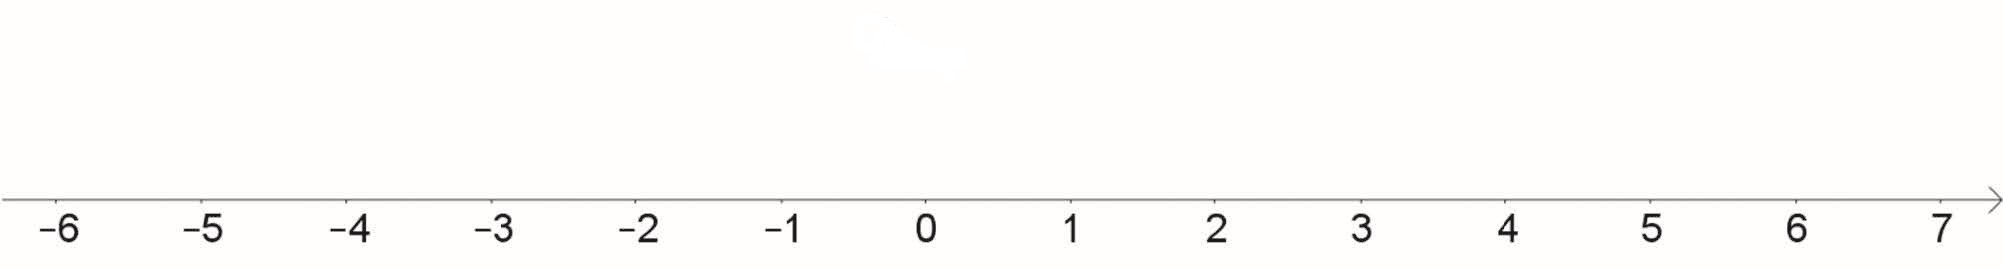
\includegraphics[width = 0.9 \textwidth]{media/Zahlengeradeo.jpg}
% \end{center}

Die imaginäre Einheit $i$ hat aber auf der Zahlengeraden keinen Platz!

Es war eine geniale und bahnbrechende Idee des Mathematikers Carl Friedrich Gauss (1777 – 1855), die Zahlengerade ins Zweidimensionale zu erweitern und der Zahl $i$ in der Ebene einen Platz oberhalb der Null zu geben:

\begin{center}
    \begin{tikzpicture}
        % Zeichne die Zahlengerade
        \draw[->] (-6.5,0) -- (7,0) node[below] {};
        
        % Markierungen für ganze Zahlen
        \foreach \x in {-6,-5,-4,-3,-2,-1,0,1,2,3,4,5,6}
            \draw (\x,0) -- (\x,-0.2) node[below] {$\x$};
        
        % Markierungen für spezielle Zahlen
        \fill[red] (0,1) circle (0.1) node[above] {$i$};



    \end{tikzpicture}
\end{center}
% \begin{center}
%     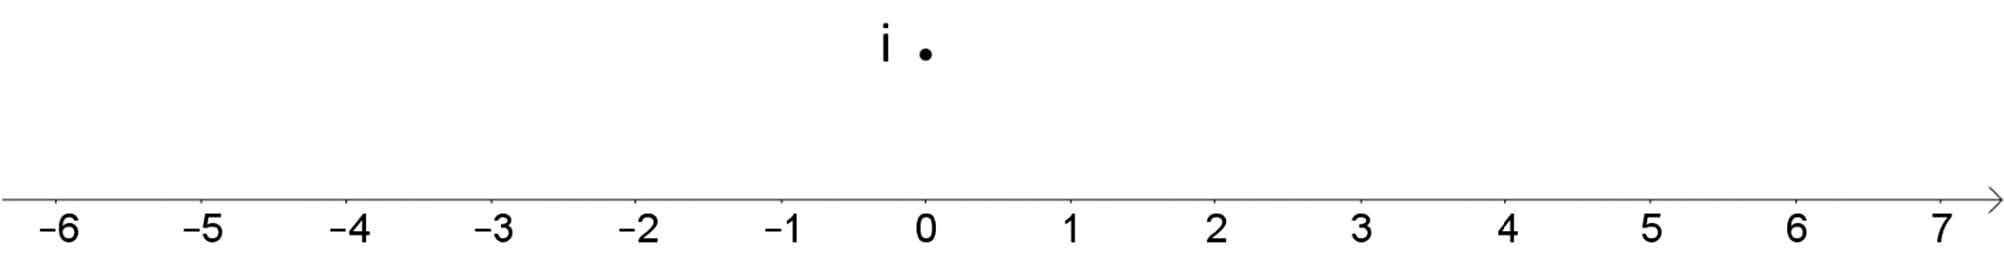
\includegraphics[width = 0.9 \textwidth]{media/Zahlengeradei.jpg}
% \end{center}

Wenn man diese Idee auf alle anderen komplexen Zahlen überträgt, erhält man die \textit{komplexe Zahlenebene} oder \textit{Gauss'sche Zahlenebene:}

\begin{center}
    \begin{tikzpicture}[scale=0.7]
        % Gitter
        \draw[dashed, very thin, gray] (-5,-5) grid (5,5);
        
        % Achsen mit Skala
        \draw[->] (-5,0) -- (5,0) node[right] {Reelle Achse};
        \draw[->] (0,-5) -- (0,5) node[right] {Imaginäre Achse};
        \foreach \x in {-4,-3,-2,-1,1,2,3,4} 
            \draw (\x,0) -- (\x,-0.2) node[below] {$\x$};
         \foreach \y in {-4,-3,-2,2,3,4}
            \draw (0,\y) -- (-0.2,\y) node[left] {$\y i$};
        \draw (0,1) -- (-0.2,1) node[left] {$i$};
        \draw (0,-1) -- (-0.2,-1) node[left] {$-i$};
        
        % Punkte und Markierungen
        %\draw[dashed, very thin, gray] (2,0) -- (2,3) -- (0,3);
        \fill[red] (0,1) circle (0.1) node[right] {$z = i$};
        \fill[purple] (2,3) circle (0.1) node[right] {$w = 2 + 3i$};
    \end{tikzpicture}
\end{center}

\clearpage
\begin{ueb}
    {Zur komplexen Zahlenebene}{}
   \begin{enumerate}
    \item Stellen Sie die nachfolgenden komplexen Zahlen in der Gauss'schen Zahlenebene dar:
    \begin{multicols}{3}
    \begin{enumerate}
        \item $2$
        \item $3i$
        \item $-2$
        \item $-4-2i$
        \item $-4+2i$
        \item $4+2i$
    \end{enumerate}
\end{multicols}
    \begin{center}
        
            \begin{tikzpicture}[scale = 0.7]
                % Gitter
                \draw[dashed, very thin, gray] (-5,-5) grid (5,5);
                
                % Achsen mit Skala
                \draw[->] (-5,0) -- (5,0) node[above] {$\RE$};
                \draw[->] (0,-5) -- (0,5) node[right] {$\IM$};
                \foreach \x in {-4,-3,-2,-1,1,2,3,4} 
                    \draw (\x,0) -- (\x,-0.2) node[below] {$\x$};
                 \foreach \y in {-4,-3,-2,2,3,4}
                    \draw (0,\y) -- (-0.2,\y) node[left] {$\y i$};
                \draw (0,1) -- (-0.2,1) node[left] {$i$};
                \draw (0,-1) -- (-0.2,-1) node[left] {$-i$};
                
                % Punkte und Markierungen
                % \draw[dashed, very thin, gray] (2,0) -- (2,3) -- (0,3);
                % \fill[red] (0,1) circle (0.1) node[right] {$z = i$};
                % \fill[purple] (2,3) circle (0.1) node[right] {$w = 2 + 3i$};
            \end{tikzpicture}
        \end{center}
    \item     Gegeben ist die komplexe Zahl $z=3+2i$. Stellen Sie die nachfolgenden komplexen Zahlen in der Gauss'schen Zahlenebene dar:
        \begin{multicols}{3}
        \begin{enumerate}
            \item $z$
            \item $-z$
            \item $\overline{z}$
            \item $-\overline{z}$
            \item $i\cdot z$
            \item $\frac{z}{i}$
        \end{enumerate}
    \end{multicols}
    \begin{center}
        
        \begin{tikzpicture}[scale = 0.7]
            % Gitter
            \draw[dashed, very thin, gray] (-5,-5) grid (5,5);
            
            % Achsen mit Skala
            \draw[->] (-5,0) -- (5,0) node[above] {$\RE$};
            \draw[->] (0,-5) -- (0,5) node[right] {$\IM$};
            \foreach \x in {-4,-3,-2,-1,1,2,3,4} 
                \draw (\x,0) -- (\x,-0.2) node[below] {$\x$};
             \foreach \y in {-4,-3,-2,2,3,4}
                \draw (0,\y) -- (-0.2,\y) node[left] {$\y i$};
            \draw (0,1) -- (-0.2,1) node[left] {$i$};
            \draw (0,-1) -- (-0.2,-1) node[left] {$-i$};
            
            % Punkte und Markierungen
            % \draw[dashed, very thin, gray] (2,0) -- (2,3) -- (0,3);
            % \fill[red] (0,1) circle (0.1) node[right] {$z = i$};
            % \fill[purple] (2,3) circle (0.1) node[right] {$w = 2 + 3i$};
        \end{tikzpicture}
    \end{center}
       
\newpage
\item Markieren Sie in der Zahlenebene die Menge aller Zahlen mit der angegebenen Eigenschaft:
        \begin{multicols}{2}
            \begin{enumerate}
                \item[\textbf{a)}] Der Imaginärteil ist 2.
                \begin{center}
        
                    \begin{tikzpicture}[scale = 0.55]
                        % Gitter
                        \draw[dashed, very thin, gray] (-5,-5) grid (5,5);
                        
                        % Achsen mit Skala
                        \draw[->] (-5,0) -- (5,0) node[above] {$\RE$};
                        \draw[->] (0,-5) -- (0,5) node[right] {$\IM$};
                        \foreach \x in {-4,-3,-2,-1,1,2,3,4} 
                            \draw (\x,0) -- (\x,-0.2) ;
                         \foreach \y in {-4,-3,-2,2,3,4}
                            \draw (0,\y) -- (-0.2,\y) ;
                        \draw (0,1) -- (-0.2,1) node[left] {$i$};
                        \draw (1,0) -- (1,-0.2) node[below] {$1$};
                        
                        % Punkte und Markierungen
                        % \draw[dashed, very thin, gray] (2,0) -- (2,3) -- (0,3);
                        % \fill[red] (0,1) circle (0.1) node[right] {$z = i$};
                        % \fill[purple] (2,3) circle (0.1) node[right] {$w = 2 + 3i$};
                    \end{tikzpicture}
                \end{center}
                
                \item[\textbf{b)}] $-1 \leq \operatorname{Re}(z) < 4$
                \begin{center}
        
                    \begin{tikzpicture}[scale = 0.55]
                        % Gitter
                        \draw[dashed, very thin, gray] (-5,-5) grid (5,5);
                        
                        % Achsen mit Skala
                        \draw[->] (-5,0) -- (5,0) node[above] {$\RE$};
                        \draw[->] (0,-5) -- (0,5) node[right] {$\IM$};
                        \foreach \x in {-4,-3,-2,-1,1,2,3,4} 
                            \draw (\x,0) -- (\x,-0.2) ;
                         \foreach \y in {-4,-3,-2, -1,2,3,4}
                            \draw (0,\y) -- (-0.2,\y) ;
                        \draw (0,1) -- (-0.2,1) node[left] {$i$};
                        \draw (1,0) -- (1,-0.2) node[below] {$1$};
                        
                        % Punkte und Markierungen
                        % \draw[dashed, very thin, gray] (2,0) -- (2,3) -- (0,3);
                        % \fill[red] (0,1) circle (0.1) node[right] {$z = i$};
                        % \fill[purple] (2,3) circle (0.1) node[right] {$w = 2 + 3i$};
                    \end{tikzpicture}
                \end{center}
                
                
                
                \item[\textbf{c)}] $\operatorname{Re}(z)^2 + \operatorname{Im}(z)^2 = 4$
                \begin{center}
        
                    \begin{tikzpicture}[scale = 0.55]
                        % Gitter
                        \draw[dashed, very thin, gray] (-5,-5) grid (5,5);
                        
                        % Achsen mit Skala
                        \draw[->] (-5,0) -- (5,0) node[above] {$\RE$};
                        \draw[->] (0,-5) -- (0,5) node[right] {$\IM$};
                        \foreach \x in {-4,-3,-2,-1,1,2,3,4} 
                            \draw (\x,0) -- (\x,-0.2) ;
                         \foreach \y in {-4,-3,-2, -1,2,3,4}
                            \draw (0,\y) -- (-0.2,\y) ;
                        \draw (0,1) -- (-0.2,1) node[left] {$i$};
                        \draw (1,0) -- (1,-0.2) node[below] {$1$};
                        
                        % Punkte und Markierungen
                        % \draw[dashed, very thin, gray] (2,0) -- (2,3) -- (0,3);
                        % \fill[red] (0,1) circle (0.1) node[right] {$z = i$};
                        % \fill[purple] (2,3) circle (0.1) node[right] {$w = 2 + 3i$};
                    \end{tikzpicture}
                \end{center}
                
                
                \item[\textbf{d)}] $\operatorname{Re}(z) = 2 \cdot \operatorname{Im}(z)$
                \begin{center}
        
                    \begin{tikzpicture}[scale = 0.55]
                        % Gitter
                        \draw[dashed, very thin, gray] (-5,-5) grid (5,5);
                        
                        % Achsen mit Skala
                        \draw[->] (-5,0) -- (5,0) node[above] {$\RE$};
                        \draw[->] (0,-5) -- (0,5) node[right] {$\IM$};
                        \foreach \x in {-4,-3,-2,-1,1,2,3,4} 
                            \draw (\x,0) -- (\x,-0.2) ;
                         \foreach \y in {-4,-3,-2, -1,2,3,4}
                            \draw (0,\y) -- (-0.2,\y) ;
                        \draw (0,1) -- (-0.2,1) node[left] {$i$};
                        \draw (1,0) -- (1,-0.2) node[below] {$1$};
                        
                        % Punkte und Markierungen
                        % \draw[dashed, very thin, gray] (2,0) -- (2,3) -- (0,3);
                        % \fill[red] (0,1) circle (0.1) node[right] {$z = i$};
                        % \fill[purple] (2,3) circle (0.1) node[right] {$w = 2 + 3i$};
                    \end{tikzpicture}
                \end{center}
                
                
                \item[\textbf{e)}] $\operatorname{Im}(\bar{z}) \geq 1$
                \begin{center}
        
                    \begin{tikzpicture}[scale = 0.55]
                        % Gitter
                        \draw[dashed, very thin, gray] (-5,-5) grid (5,5);
                        
                        % Achsen mit Skala
                        \draw[->] (-5,0) -- (5,0) node[above] {$\RE$};
                        \draw[->] (0,-5) -- (0,5) node[right] {$\IM$};
                        \foreach \x in {-4,-3,-2,-1,1,2,3,4} 
                            \draw (\x,0) -- (\x,-0.2) ;
                         \foreach \y in {-4,-3,-2, -1,2,3,4}
                            \draw (0,\y) -- (-0.2,\y) ;
                        \draw (0,1) -- (-0.2,1) node[left] {$i$};
                        \draw (1,0) -- (1,-0.2) node[below] {$1$};
                        
                        % Punkte und Markierungen
                        % \draw[dashed, very thin, gray] (2,0) -- (2,3) -- (0,3);
                        % \fill[red] (0,1) circle (0.1) node[right] {$z = i$};
                        % \fill[purple] (2,3) circle (0.1) node[right] {$w = 2 + 3i$};
                    \end{tikzpicture}
                \end{center}
                
                
                
                \item[\textbf{f)}] $(\operatorname{Re}(z) + \operatorname{Im}(z))^2 = 1$
                \begin{center}
        
                    \begin{tikzpicture}[scale = 0.55]
                        % Gitter
                        \draw[dashed, very thin, gray] (-5,-5) grid (5,5);
                        
                        % Achsen mit Skala
                        \draw[->] (-5,0) -- (5,0) node[above] {$\RE$};
                        \draw[->] (0,-5) -- (0,5) node[right] {$\IM$};
                        \foreach \x in {-4,-3,-2,-1,1,2,3,4} 
                            \draw (\x,0) -- (\x,-0.2) ;
                         \foreach \y in {-4,-3,-2, -1,2,3,4}
                            \draw (0,\y) -- (-0.2,\y) ;
                        \draw (0,1) -- (-0.2,1) node[left] {$i$};
                        \draw (1,0) -- (1,-0.2) node[below] {$1$};
                        
                        % Punkte und Markierungen
                        % \draw[dashed, very thin, gray] (2,0) -- (2,3) -- (0,3);
                        % \fill[red] (0,1) circle (0.1) node[right] {$z = i$};
                        % \fill[purple] (2,3) circle (0.1) node[right] {$w = 2 + 3i$};
                    \end{tikzpicture}
                \end{center}
                
                
            \end{enumerate}
            \end{multicols}
        \end{enumerate}
            
\end{ueb}


\clearpage
\emph{Lösungen}
\begin{enumerate}
    \item Stellen Sie die nachfolgenden komplexen Zahlen in der Gauss'schen Zahlenebene dar:
      \begin{center}
        
            \begin{tikzpicture}[scale = 0.7]
                % Gitter
                \draw[dashed, very thin, gray] (-5,-5) grid (5,5);
                
                % Achsen mit Skala
                \draw[->] (-5,0) -- (5,0) node[above] {$\RE$};
                \draw[->] (0,-5) -- (0,5) node[right] {$\IM$};
                \foreach \x in {-4,-3,-2,-1,1,2,3,4} 
                    \draw (\x,0) -- (\x,-0.2) node[below] {$\x$};
                 \foreach \y in {-4,-3,-2,2,3,4}
                    \draw (0,\y) -- (-0.2,\y) node[left] {$\y i$};
                \draw (0,1) -- (-0.2,1) node[left] {$i$};
                \draw (0,-1) -- (-0.2,-1) node[left] {$-i$};
                
                % Punkte und Markierungen
                \fill[red] (2,0) circle (0.1) node[above] {$2$};
                \fill[red] (0,3) circle (0.1) node[right] {$3i$};
                \fill[red] (-2,0) circle (0.1) node[above] {$-2$};
                \fill[red] (-4,-2) circle (0.1) node[below] {$-4-2i$};
                \fill[red] (-4,2) circle (0.1) node[above] {$-4+2i$};
                \fill[red] (4,2) circle (0.1) node[above] {$4+2i$};
            \end{tikzpicture}
        \end{center}
    \item     Gegeben ist die komplexe Zahl $z=3+2i$. Stellen Sie die nachfolgenden komplexen Zahlen in der Gauss'schen Zahlenebene dar:
        
    \begin{center}
        
        \begin{tikzpicture}[scale = 0.7]
            % Gitter
            \draw[dashed, very thin, gray] (-5,-5) grid (5,5);
            
            % Achsen mit Skala
            \draw[->] (-5,0) -- (5,0) node[above] {$\RE$};
            \draw[->] (0,-5) -- (0,5) node[right] {$\IM$};
            \foreach \x in {-4,-3,-2,-1,1,2,3,4} 
                \draw (\x,0) -- (\x,-0.2) node[below] {$\x$};
             \foreach \y in {-4,-3,-2,2,3,4}
                \draw (0,\y) -- (-0.2,\y) node[left] {$\y i$};
            \draw (0,1) -- (-0.2,1) node[left] {$i$};
            \draw (0,-1) -- (-0.2,-1) node[left] {$-i$};
            
            % Punkte und Markierungen
            \fill[red] (3,2) circle (0.1) node[above right] {$z$};
            \fill[red] (-3,-2) circle (0.1) node[below left] {$-z$};
            \fill[red] (3,-2) circle (0.1) node[below right] {$\overline{z}$};
            \fill[red] (-3,2) circle (0.1) node[above left] {$-\overline{z}$};
            \fill[red] (-2,3) circle (0.1) node[above left] {$i \cdot z$};
            \fill[red] (2,-3) circle (0.1) node[below right] {$\frac{z}{i}$};
        \end{tikzpicture}
    \end{center}
       
\newpage
\item Markieren Sie in der Zahlenebene die Menge aller Zahlen mit der angegebenen Eigenschaft:
        \begin{multicols}{2}
            \begin{enumerate}
                \item[\textbf{a)}] Der Imaginärteil ist 2.
                \begin{center}
        
                    \begin{tikzpicture}[scale = 0.55]
                        % Gitter
                        \draw[dashed, very thin, gray] (-5,-5) grid (5,5);
                        
                        % Achsen mit Skala
                        \draw[->] (-5,0) -- (5,0) node[above] {$\RE$};
                        \draw[->] (0,-5) -- (0,5) node[right] {$\IM$};
                        \foreach \x in {-4,-3,-2,-1,1,2,3,4} 
                            \draw (\x,0) -- (\x,-0.2) ;
                         \foreach \y in {-4,-3,-2, -1,2,3,4}
                            \draw (0,\y) -- (-0.2,\y) ;
                        \draw (0,1) -- (-0.2,1) node[left] {$i$};
                        \draw (1,0) -- (1,-0.2) node[below] {$1$};
                        
                        % Punkte und Markierungen
                        \draw[thick, red] (-5,2) -- (5,2);
            
                    \end{tikzpicture}
                \end{center}
                
                \item[\textbf{b)}] $-1 \leq \operatorname{Re}(z) < 4$
                \begin{center}
        
                    \begin{tikzpicture}[scale = 0.55]
                        % Gitter
                        \draw[dashed, very thin, gray] (-5,-5) grid (5,5);
                        
                        % Achsen mit Skala
                        \draw[->] (-5,0) -- (5,0) node[above] {$\RE$};
                        \draw[->] (0,-5) -- (0,5) node[right] {$\IM$};
                        \foreach \x in {-4,-3,-2,-1,1,2,3,4} 
                            \draw (\x,0) -- (\x,-0.2) ;
                         \foreach \y in {-4,-3,-2, -1,2,3,4}
                            \draw (0,\y) -- (-0.2,\y) ;
                        \draw (0,1) -- (-0.2,1) node[left] {$i$};
                        \draw (1,0) -- (1,-0.2) node[below] {$1$};
                        
                        % Punkte und Markierungen
                        \draw[thick, blue] (-1,-5) -- (-1,5);
                        %\draw[thick, blue] (4,-5) -- (4,5);
                        \fill[blue!20, opacity=0.5] (-1,-5) -- (-1,5) -- (4,5) -- (4,-5) -- cycle;
                    \end{tikzpicture}
                \end{center}
                
                
                
                \item[\textbf{c)}] $\operatorname{Re}(z)^2 + \operatorname{Im}(z)^2 = 4$
                \begin{center}
        
                    \begin{tikzpicture}[scale = 0.55]
                        % Gitter
                        \draw[dashed, very thin, gray] (-5,-5) grid (5,5);
                        
                        % Achsen mit Skala
                        \draw[->] (-5,0) -- (5,0) node[above] {$\RE$};
                        \draw[->] (0,-5) -- (0,5) node[right] {$\IM$};
                        \foreach \x in {-4,-3,-2,-1,1,2,3,4} 
                            \draw (\x,0) -- (\x,-0.2) ;
                         \foreach \y in {-4,-3,-2, -1,2,3,4}
                            \draw (0,\y) -- (-0.2,\y) ;
                        \draw (0,1) -- (-0.2,1) node[left] {$i$};
                        \draw (1,0) -- (1,-0.2) node[below] {$1$};
                        
                        % Punkte und Markierungen
                        \draw[thick, red] (0,0) circle (2);
            
                    \end{tikzpicture}
                \end{center}
                
                
                \item[\textbf{d)}] $\operatorname{Re}(z) = 2 \cdot \operatorname{Im}(z)$
                \begin{center}
        
                    \begin{tikzpicture}[scale = 0.55]
                        % Gitter
                        \draw[dashed, very thin, gray] (-5,-5) grid (5,5);
                        
                        % Achsen mit Skala
                        \draw[->] (-5,0) -- (5,0) node[above] {$\RE$};
                        \draw[->] (0,-5) -- (0,5) node[right] {$\IM$};
                        \foreach \x in {-4,-3,-2,-1,1,2,3,4} 
                            \draw (\x,0) -- (\x,-0.2) ;
                         \foreach \y in {-4,-3,-2, -1,2,3,4}
                            \draw (0,\y) -- (-0.2,\y) ;
                        \draw (0,1) -- (-0.2,1) node[left] {$i$};
                        \draw (1,0) -- (1,-0.2) node[below] {$1$};
                        
                        % Punkte und Markierungen
                        \draw[thick, orange] (-5,-2.5) -- (5,2.5);
                    \end{tikzpicture}
                \end{center}
                
                
                \item[\textbf{e)}] $\operatorname{Im}(\bar{z}) \geq 1$
                \begin{center}
        
                    \begin{tikzpicture}[scale = 0.55]
                        % Gitter
                        \draw[dashed, very thin, gray] (-5,-5) grid (5,5);
                        
                        % Achsen mit Skala
                        \draw[->] (-5,0) -- (5,0) node[above] {$\RE$};
                        \draw[->] (0,-5) -- (0,5) node[right] {$\IM$};
                        \foreach \x in {-4,-3,-2,-1,1,2,3,4} 
                            \draw (\x,0) -- (\x,-0.2) ;
                         \foreach \y in {-4,-3,-2, -1,2,3,4}
                            \draw (0,\y) -- (-0.2,\y) ;
                        \draw (0,1) -- (-0.2,1) node[left] {$i$};
                        \draw (1,0) -- (1,-0.2) node[below] {$1$};
                        
                        % Punkte und Markierungen
                        %\draw[thick, purple] (-5,-1) -- (5,-1);
                        \fill[purple!20, opacity=0.5] (-5,-1) -- (5,-1) -- (5,-5) -- (-5,-5) -- cycle;
                        \draw[thick, purple] (-5,-1) -- (5,-1);
                    \end{tikzpicture}
                \end{center}
                
                
                
                \item[\textbf{f)}] $(\operatorname{Re}(z) + \operatorname{Im}(z))^2 = 1$
                \begin{center}
        
                    \begin{tikzpicture}[scale = 0.55]
                        % Gitter
                        \draw[dashed, very thin, gray] (-5,-5) grid (5,5);
                        
                        % Achsen mit Skala
                        \draw[->] (-5,0) -- (5,0) node[above] {$\RE$};
                        \draw[->] (0,-5) -- (0,5) node[right] {$\IM$};
                        \foreach \x in {-4,-3,-2,-1,1,2,3,4} 
                            \draw (\x,0) -- (\x,-0.2) ;
                         \foreach \y in {-4,-3,-2, -1,2,3,4}
                            \draw (0,\y) -- (-0.2,\y) ;
                        \draw (0,1) -- (-0.2,1) node[left] {$i$};
                        \draw (1,0) -- (1,-0.2) node[below] {$1$};
                        
                        % Punkte und Markierungen
                        \draw[thick, purple] (-5,4) -- (4,-5);
                        \draw[thick, purple] (-4,5) -- (5,-4);
                    \end{tikzpicture}
                \end{center}
                
                
            \end{enumerate}
            \end{multicols}
        \end{enumerate}
            




















































\clearpage
\subsection{Der Betrag komplexer Zahlen}
Das Konzept des Betrags einer reellen Zahl kann auf komplexe Zahlen erweitert werden, indem der Betrag einer komplexen Zahl als deren Abstand zum Ursprung in der komplexen Zahlenebene definiert wird.
\begin{center}
    \begin{tikzpicture}[scale = 0.7]
        % Gitter
        \draw[dashed, very thin, very thin, gray] (-5,-5) grid (5,5);
        
        % Achsen mit Skala
        \draw[->] (-5,0) -- (5,0) node[above] {Reelle Achse};
        \draw[->] (0,-5) -- (0,5) node[right] {Imaginäre Achse};
        \foreach \x in {-4,-3,-2,-1,1,2,3,4} 
            \draw (\x,0) -- (\x,-0.2) node[below] {$\x$};
         \foreach \y in {-4,-3,-2,2,3,4}
            \draw (0,\y) -- (-0.2,\y) node[left] {$\y i$};
        \draw (0,1) -- (-0.2,1) node[left] {$i$};
        \draw (0,-1) -- (-0.2,-1) node[left] {$-i$};
        % Punkte und Markierungen
         \fill[red] (-3,0) circle (0.1) node[above] {$z = -3$};
         \fill[purple] (2,3) circle (0.1) node[right] {$w = 2 + 3i$};
    \end{tikzpicture}
\end{center}

\begin{definition}
    {Der Betrag einer komplexen Zahl}{}
    Der \emph{Betrag} einer komplexen Zahl $z=a+bi$ entspricht dem Abstand von $z$ zum Urspung $O(0, 0)$ in der komplexen Zahlenebene. Der Betrag von $z=a+bi$ wird so berechnet: 

$$|z|=|a+bi|=\ldots\ldots$$

\end{definition}

\begin{ueb}
    {}{}
    \begin{enumerate}
        \item  Gegeben sind $v=-3-4i$, $w=-2i$ und $z=1+i$. Berechnen Sie
        \begin{enumerate}
            \item $|z|=$
            \vfill
            \item $|\overline{w}|=$
            \vfill
            \item $|2v|=$
            \vfill
            \item $\left|\frac{v}{z}\right|=$
            \vfill
            \item $\left|w\cdot v\right|=$
            \vfill
        \end{enumerate}
        \item Zeigen Sie, dass für alle $z\in \C$ gilt: $z\cdot \overline{z}=|z|^2$.
        \item Zeigen Sie, dass $|z-w|$ dem Abstand der beiden Zahlen $z$ und $w$ in der komplexe Zahlenebene entspricht.
        \item Markieren Sie in der Gauss'schen Zahlenebene jeweils alle komplexe Zahlen $z$ mit folgender Eigenschaft:

        \begin{multicols}{2}
        \begin{enumerate}
            \item $|z|<3$
            \begin{center}
        
                \begin{tikzpicture}[scale = 0.55]
                    % Gitter
                    \draw[dashed, very thin, gray] (-5,-5) grid (5,5);
                    
                    % Achsen mit Skala
                    \draw[->] (-5,0) -- (5,0) node[above] {$\RE$};
                    \draw[->] (0,-5) -- (0,5) node[right] {$\IM$};
                    \foreach \x in {-4,-3,-2,-1,1,2,3,4} 
                        \draw (\x,0) -- (\x,-0.2) ;
                     \foreach \y in {-4,-3,-2, -1,2,3,4}
                        \draw (0,\y) -- (-0.2,\y) ;
                    \draw (0,1) -- (-0.2,1) node[left] {$i$};
                    \draw (1,0) -- (1,-0.2) node[below] {$1$};
                    
                    % Punkte und Markierungen
                    % \draw[dashed, very thin, gray] (2,0) -- (2,3) -- (0,3);
                    % \fill[red] (0,1) circle (0.1) node[right] {$z = i$};
                    % \fill[purple] (2,3) circle (0.1) node[right] {$w = 2 + 3i$};
                \end{tikzpicture}
            \end{center}
            
            \item $\IM(z)=|z|$
            \begin{center}
        
                \begin{tikzpicture}[scale = 0.55]
                    % Gitter
                    \draw[dashed, very thin, gray] (-5,-5) grid (5,5);
                    
                    % Achsen mit Skala
                    \draw[->] (-5,0) -- (5,0) node[above] {$\RE$};
                    \draw[->] (0,-5) -- (0,5) node[right] {$\IM$};
                    \foreach \x in {-4,-3,-2,-1,1,2,3,4} 
                        \draw (\x,0) -- (\x,-0.2) ;
                     \foreach \y in {-4,-3,-2, -1,2,3,4}
                        \draw (0,\y) -- (-0.2,\y) ;
                    \draw (0,1) -- (-0.2,1) node[left] {$i$};
                    \draw (1,0) -- (1,-0.2) node[below] {$1$};
                    
                    % Punkte und Markierungen
                    % \draw[dashed, very thin, gray] (2,0) -- (2,3) -- (0,3);
                    % \fill[red] (0,1) circle (0.1) node[right] {$z = i$};
                    % \fill[purple] (2,3) circle (0.1) node[right] {$w = 2 + 3i$};
                \end{tikzpicture}
            
            \end{center}

            \item $|z- 3| = 2$
            \begin{center}
        
                \begin{tikzpicture}[scale = 0.55]
                    % Gitter
                    \draw[dashed, very thin, gray] (-5,-5) grid (5,5);
                    
                    % Achsen mit Skala
                    \draw[->] (-5,0) -- (5,0) node[above] {$\RE$};
                    \draw[->] (0,-5) -- (0,5) node[right] {$\IM$};
                    \foreach \x in {-4,-3,-2,-1,1,2,3,4} 
                        \draw (\x,0) -- (\x,-0.2) ;
                     \foreach \y in {-4,-3,-2, -1,2,3,4}
                        \draw (0,\y) -- (-0.2,\y) ;
                    \draw (0,1) -- (-0.2,1) node[left] {$i$};
                    \draw (1,0) -- (1,-0.2) node[below] {$1$};
                    
                    % Punkte und Markierungen
                    % \draw[dashed, very thin, gray] (2,0) -- (2,3) -- (0,3);
                    % \fill[red] (0,1) circle (0.1) node[right] {$z = i$};
                    % \fill[purple] (2,3) circle (0.1) node[right] {$w = 2 + 3i$};
                \end{tikzpicture}
            \end{center}

            
            \item $|z+i|\geq 2$
            \begin{center}
        
                \begin{tikzpicture}[scale = 0.55]
                    % Gitter
                    \draw[dashed, very thin, gray] (-5,-5) grid (5,5);
                    
                    % Achsen mit Skala
                    \draw[->] (-5,0) -- (5,0) node[above] {$\RE$};
                    \draw[->] (0,-5) -- (0,5) node[right] {$\IM$};
                    \foreach \x in {-4,-3,-2,-1,1,2,3,4} 
                        \draw (\x,0) -- (\x,-0.2) ;
                     \foreach \y in {-4,-3,-2, -1,2,3,4}
                        \draw (0,\y) -- (-0.2,\y) ;
                    \draw (0,1) -- (-0.2,1) node[left] {$i$};
                    \draw (1,0) -- (1,-0.2) node[below] {$1$};
                    
                    % Punkte und Markierungen
                    % \draw[dashed, very thin, gray] (2,0) -- (2,3) -- (0,3);
                    % \fill[red] (0,1) circle (0.1) node[right] {$z = i$};
                    % \fill[purple] (2,3) circle (0.1) node[right] {$w = 2 + 3i$};
                \end{tikzpicture}
            \end{center}
            
        \end{enumerate}
        \end{multicols}
        \item Sind die folgenden Aussagen wahr oder falsch? Begründen Sie:

        \begin{enumerate}
            \item Für alle $w,z\in \C$ gilt: $|w\cdot z|=|w|\cdot |z|$.
            \vfill
            \item Für alle $w,z\in \C$ gilt: $|w + z|=|w|+|z|$.
            \vfill
            \item Für alle $z\in \C$ gilt: $|z|=|\overline{z}|$.
            \vfill
        \end{enumerate}
        
    \end{enumerate}
\end{ueb}


\begin{ueb}
    {Programmieraufgabe}{}
    Ergänzen Sie den Konstruktor \lstinline{__init__()} der Klasse `komplex' um das Attribut \lstinline{self.betrag}, worin der Betrag der komplexen Zahl gespeichert wird, sodass man mit \lstinline{z.betrag} den Betrag der Zahl $z$ erhält.



    Für die Berechnung der Wurzel müssen Sie die entsprechende Funktion zuerst importieren: \lstinline{from math import sqrt}
\end{ueb}


\clearpage
\emph{Lösungen}
\begin{enumerate}

\item Gegeben sind $v=-3-4i$, $w=-2i$ und $z=1+i$. Berechnen Sie:
    \begin{enumerate}
        \item $|z|= \sqrt{2}$
        \item $|\overline{w}|= 2$
        \item $|2v|= 10$
        \item $\left|\frac{v}{z}\right|= \frac{5\sqrt{2}}{2}$
        \item $\left|w\cdot v\right|= 10$
    \end{enumerate}
    
    \item  $z\cdot \overline{z}= (a+bi)(a-bi) = a^2+b^2 = |z|^2$.
    
    \item Rechne $|z-w|= |(a+bi)-(c+di)| = \cdots = \sqrt{(a-c)^2+(b-d)^2}$. Vergleiche mit der Berechnung des Abstands der beiden Punkte mit Pythagoras.
    \item Markieren Sie in der Gauss'schen Zahlenebene jeweils alle komplexe Zahlen $z$ mit folgender Eigenschaft:

        \begin{multicols}{2}
        \begin{enumerate}
            \item $|z|<3$
            \begin{center}
        
                \begin{tikzpicture}[scale = 0.55]
                    % Gitter
                    \draw[dashed, very thin, gray] (-5,-5) grid (5,5);
                    
                    % Achsen mit Skala
                    \draw[->] (-5,0) -- (5,0) node[above] {$\RE$};
                    \draw[->] (0,-5) -- (0,5) node[right] {$\IM$};
                    \foreach \x in {-4,-3,-2,-1,1,2,3,4} 
                        \draw (\x,0) -- (\x,-0.2) ;
                     \foreach \y in {-4,-3,-2, -1,2,3,4}
                        \draw (0,\y) -- (-0.2,\y) ;
                    \draw (0,1) -- (-0.2,1) node[left] {$i$};
                    \draw (1,0) -- (1,-0.2) node[below] {$1$};
                    
                    % Punkte und Markierungen
                    \fill[purple!20, opacity=0.5] (0,0) circle (3);
                \end{tikzpicture}
            \end{center}
            
            \item $\IM(z)=|z|$
            \begin{center}
        
                \begin{tikzpicture}[scale = 0.55]
                    % Gitter
                    \draw[dashed, very thin, gray] (-5,-5) grid (5,5);
                    
                    % Achsen mit Skala
                    \draw[->] (-5,0) -- (5,0) node[above] {$\RE$};
                    \draw[->] (0,-5) -- (0,5) node[right] {$\IM$};
                    \foreach \x in {-4,-3,-2,-1,1,2,3,4} 
                        \draw (\x,0) -- (\x,-0.2) ;
                     \foreach \y in {-4,-3,-2, -1,2,3,4}
                        \draw (0,\y) -- (-0.2,\y) ;
                    \draw (0,1) -- (-0.2,1) node[left] {$i$};
                    \draw (1,0) -- (1,-0.2) node[below] {$1$};
                    
                    % Punkte und Markierungen
                    \draw[thick, purple] (0,0) -- (0,5);
                    \fill[purple] (0,0) circle (0.1) ;                    
                \end{tikzpicture}
            
            \end{center}

            \item $|z- 3| = 2$
            \begin{center}
        
                \begin{tikzpicture}[scale = 0.55]
                    % Gitter
                    \draw[dashed, very thin, gray] (-5,-5) grid (5,5);
                    
                    % Achsen mit Skala
                    \draw[->] (-5,0) -- (5,0) node[above] {$\RE$};
                    \draw[->] (0,-5) -- (0,5) node[right] {$\IM$};
                    \foreach \x in {-4,-3,-2,-1,1,2,3,4} 
                        \draw (\x,0) -- (\x,-0.2) ;
                     \foreach \y in {-4,-3,-2, -1,2,3,4}
                        \draw (0,\y) -- (-0.2,\y) ;
                    \draw (0,1) -- (-0.2,1) node[left] {$i$};
                    \draw (1,0) -- (1,-0.2) node[below] {$1$};
                    
                    % Punkte und Markierungen
                    \draw[thick, purple] (3,0) circle (2);
                \end{tikzpicture}
            \end{center}

            
            \item $|z+i|\geq 2$
            \begin{center}
        
                \begin{tikzpicture}[scale = 0.55, even odd rule]
                    % Gitter
                    \draw[dashed, very thin, gray] (-5,-5) grid (5,5);
                    
                    % Achsen mit Skala
                    \draw[->] (-5,0) -- (5,0) node[above] {$\RE$};
                    \draw[->] (0,-5) -- (0,5) node[right] {$\IM$};
                    \foreach \x in {-4,-3,-2,-1,1,2,3,4} 
                        \draw (\x,0) -- (\x,-0.2) ;
                     \foreach \y in {-4,-3,-2, -1,2,3,4}
                        \draw (0,\y) -- (-0.2,\y) ;
                    \draw (0,1) -- (-0.2,1) node[left] {$i$};
                    \draw (1,0) -- (1,-0.2) node[below] {$1$};
                    
                    % % Punkte und Markierungen
                    \fill[even odd rule, purple!30, opacity=0.5] (-5,-5) rectangle (5,5) (0,-1) circle (2);
                    \draw[thick, purple] (0,-1) circle (2);

                \end{tikzpicture}
            \end{center}
            
        \end{enumerate}
        \end{multicols}
        \item Sind die folgenden Aussagen wahr oder falsch? 

        \begin{enumerate}
            \item Für alle $w,z\in \C$ gilt: $|w\cdot z|=|w|\cdot |z|$. Setze $z=a+bi, w=c+di$ und rechne \dots WAHR.
            
            \item Für alle $w,z\in \C$ gilt: $|w + z|=|w|+|z|$. Gegenbeispiel $z=1, w=-1$.
            \item Für alle $z\in \C$ gilt: $|z|=|\overline{z}|$. Setze $z=a+bi$ und rechne \dots WAHR.
        \end{enumerate}
        

\end{enumerate}
















































\clearpage
\subsection{Geometrische Interpretation der Grundoperationen}
Die Summe $z+w$, die Differenz $z-w$ und das Produkt $z\cdot w$ zweier komplexer Zahlen haben in der Gauss'schen Zahlenebene eine elegante geometrische Interpretation. Um diese zu sehen, müssen wir aber zuerst die komplexen Zahlen als Ortsvektoren verstehen.

Genauer: wir interpretieren die komplexe Zahl $z=a+bi$ als den Ortsvektor $\vec{z}=\left(\begin{array}{c}a\\b\\ \end{array}\right)$.

Die Addition, Subtraktion und die reellen Vielfache von komplexen Zahlen entspricht dann der analogen Operation für Vektoren.

\begin{multicols}{2}

    \begin{center}

        Addition

        \begin{tikzpicture}[scale = 1.2]
      
            
            % Achsen mit Skala
            \draw[->, thick] (-1.5,0) -- (4.5,0) node[above] {$\RE$};
            \draw[->, thick] (0,-1.5) -- (0,2.5) node[right] {$\IM$};
            \foreach \x in {-1,2,3,4} 
                \draw (\x,0.1) -- (\x,-0.1) ;
            \foreach \y in {-1,2,} 
                \draw (0.1,\y) -- (-0.1,\y) ;
            \draw (0.1,1) -- (-0.1,1) node[left] {$i$};
            \draw (1,0.1) -- (1,-0.1) node[below] {$1$};
            
             % Vektoren
             \draw[->, thick, dashed] (0,0) -- node[above] {$\vec{z}_1$} ++(1,5/4) node[above left, ForestGreen] {$z_1 = a + bi$};
             \draw[->, thick, dashed] (0,0) -- node[below right] {$\vec{z}_2$} ++(2,3/4) node[below right, ForestGreen] {$z_2 = c + di$};
             \draw[->, thick, orange] (0,0) -- (3,2) node[above right, orange] {$z_1 + z_2$};
             \draw[->, thick, dashed] (1,5/4) -- (3,2) ; 
             \draw[->, thick, dashed] (2,3/4) -- (3,2) ; 
            
             % Punkte
             \fill[ForestGreen] (1,5/4) circle (0.05);
             \fill[ForestGreen] (2,3/4) circle (0.05) ;
             \fill[orange] (3,2) circle (0.05);
        \end{tikzpicture}
        
    \end{center}

    \begin{center}
        
        Multiplikation mit einer reellen Zahl

        \begin{tikzpicture}[scale = 1.2]
      
            
            % Achsen mit Skala
            \draw[->, thick] (-1.5,0) -- (4.5,0) node[above] {$\RE$};
            \draw[->, thick] (0,-1.5) -- (0,2.5) node[right] {$\IM$};
            \foreach \x in {-1,2,3,4} 
                \draw (\x,0.1) -- (\x,-0.1) ;
            \foreach \y in {-1,2,} 
                \draw (0.1,\y) -- (-0.1,\y) ;
            \draw (0.1,1) -- (-0.1,1) node[left] {$i$};
            \draw (1,0.1) -- (1,-0.1) node[below] {$1$};
            
             % Vektoren
             \draw[->, very thick] (0,0) -- node[above] {$\vec{z}$} ++(2,1) node[below right, ForestGreen] {$z = a + bi$};
             \draw[->, thick, orange] (0,0) -- node[above left] {$k\cdot\vec{z}$}(4,2) node[above right, orange] {$k\cdot z$};
             
        
             
          
            
             % Punkte
             \fill[ForestGreen] (2,1) circle (0.05);
             \fill[orange] (4,2) circle (0.05);
        \end{tikzpicture}
        
    \end{center}


    \begin{center}
        
  
    Subtraktion
    
    \begin{tikzpicture}[scale = 1.2]
  
        
        % Achsen mit Skala
        \draw[->, thick] (-1.5,0) -- (4.5,0) node[above] {$\RE$};
        \draw[->, thick] (0,-1.5) -- (0,2.5) node[right] {$\IM$};
        \foreach \x in {-1,2,3,4} 
            \draw (\x,0.1) -- (\x,-0.1) ;
        \foreach \y in {-1,2,} 
            \draw (0.1,\y) -- (-0.1,\y) ;
        \draw (0.1,1) -- (-0.1,1) node[left] {$i$};
        \draw (1,0.1) -- (1,-0.1) node[below] {$1$};
        
         % Vektoren
         \draw[->, thick, dashed] (0,0) -- node[left] {$\vec{z}_1$}  ++(2, 2.5) node[above, ForestGreen] {$z_1 = a + bi$};
         \draw[->, thick, dashed] (0,0) -- node[below right] {$\vec{z}_2$}  ++ (3,1.5) node[below right, ForestGreen] {$z_2 = c + di$};
         \draw[->, thick, orange] (0,0) -- (-1,1) node[above left, orange] {$z_1 - z_2$};
         \draw[->, thick, dashed] (2,2.5) -- node[above] {$-\vec{z}_2$}  ++(-3,-1.5) ; 
         \draw[->, thick, dashed] (3,1.5) -- (2,2.5) ; 
         
         % Punkte
         \fill[ForestGreen] (2,2.5) circle (0.05);
         \fill[ForestGreen] (3,1.5) circle (0.05);
         \fill[orange] (-1,1) circle (0.05);
    \end{tikzpicture}
    
\end{center}

\begin{center}
        
  
    Betrag
    
    \begin{tikzpicture}[scale = 1.2]
  
        
        % Achsen mit Skala
        \draw[->, thick] (-1.5,0) -- (4.5,0) node[above] {$\RE$};
        \draw[->, thick] (0,-1.5) -- (0,2.5) node[right] {$\IM$};
        \foreach \x in {-1,2,3,4} 
            \draw (\x,0.1) -- (\x,-0.1) ;
        \foreach \y in {-1,2,} 
            \draw (0.1,\y) -- (-0.1,\y) ;
        \draw (0.1,1) -- (-0.1,1) node[left] {$i$};
        \draw (1,0.1) -- (1,-0.1) node[below] {$1$};
        
         % Vektoren
         \draw[->, thick] (0,0) -- node[above] {$|z|$}  ++(2.5, 2) ;
         \draw[thick, orange] (0,0) -- node[below, orange] {$a$} ++(2.5,0) ;
         \draw[thick, orange] (2.5,0) -- node[right, orange] {$b$} ++(0,2);
              
         % Punkte
         \fill[ForestGreen] (2.5,2) circle (0.05) node[above, ForestGreen] {$z = a + bi$};
         
    \end{tikzpicture}
    
\end{center}

    


    
\end{multicols}

\clearpage
\begin{ueb}
    {}{}
    Gegeben sind zwei komplexe Zahlen $z$ und $w$. Bestimmen Sie die Summe $z+w$ und die Differenzen $z-w$, $w-2\bar{z}$ und $w-\frac{1}{2}z$ geometrisch durch Verknüpfen von Vektoren.

    \begin{center}
        
        \begin{tikzpicture}[scale = 1]
            % Gitter
            %\draw[dashed, very thin, gray] (-5,-5) grid (5,5);
            
            % Achsen mit Skala
            \draw[->, thick] (-5,0) -- (5,0) node[above] {$\RE$};
            \draw[->, thick] (0,-5) -- (0,5) node[right] {$\IM$};
            %\foreach \x in {-4,-3,-2,-1,1,2,3,4} 
            %    \draw (\x,0) -- (\x,-0.2) ;
            % \foreach \y in {-4,-3,-2, -1,2,3,4}
            %    \draw (0,\y) -- (-0.2,\y) ;
            %\draw (0,1) -- (-0.2,1) node[left] {$i$};
            %\draw (1,0) -- (1,-0.2) node[below] {$1$};
            
            % Punkte und Markierungen
            \fill[ForestGreen] (3,2) circle (0.1) node[left] {$z$};
            \fill[ForestGreen] (1,-2) circle (0.1) node[left] {$w$};

            %\fill[red] (4,0) circle (0.1) node[above] {z+w}
        \end{tikzpicture}
    \end{center}

\end{ueb}


\clearpage
\emph{Lösung}
\begin{center}
        
    \begin{tikzpicture}[scale = 1]
        % Gitter
        %\draw[dashed, very thin, gray] (-5,-5) grid (5,5);
        
        % Achsen mit Skala
        \draw[->, thick] (-5,0) -- (5,0) node[above] {$\RE$};
        \draw[->, thick] (0,-5) -- (0,5) node[right] {$\IM$};
        %\foreach \x in {-4,-3,-2,-1,1,2,3,4} 
        %    \draw (\x,0) -- (\x,-0.2) ;
        % \foreach \y in {-4,-3,-2, -1,2,3,4}
        %    \draw (0,\y) -- (-0.2,\y) ;
        %\draw (0,1) -- (-0.2,1) node[left] {$i$};
        %\draw (1,0) -- (1,-0.2) node[below] {$1$};
        
        % Punkte und Markierungen
        \fill[ForestGreen] (3,2) circle (0.1) node[left] {$z$};
        \fill[ForestGreen] (1,-2) circle (0.1) node[left] {$w$};

        \fill[red] (4,0) circle (0.1) node[above] {$z+w$};
        \fill[red] (2,4) circle (0.1) node[above] {$z-w$};
        \fill[red] (-0.5,-3) circle (0.1) node[above] {$w-\frac{1}{2}z$};
        \fill[red] (-5,2) circle (0.1) node[above] {$w-2\bar z$};
    \end{tikzpicture}
\end{center}





















\clearpage
\subsection{Die Polarform}

Ein Punkt in einem 2-dimensionalen Koordinatensystem ist durch die Angabe seiner kartesischen Koordinaten $x$ und $y$ eindeutig bestimmt. Ein Punkt kann auch durch den Winkel $\varphi$ (von der positiven $x$-Achse aus im Gegenuhrzeigersinn gemessen) und den Abstand $r$ (vom Ursprung) eindeutig bestimmt werden. Diese Darstellung heisst Polardarstellung.

\begin{center}
    \begin{tikzpicture}[scale = 0.7]
        % Achsen mit Skala
        \draw[->, thick] (-1.5,0) -- (4.5,0) node[above] {$\operatorname{Re}$};
        \draw[->, thick] (0,-1.5) -- (0,2.5) node[right] {$\operatorname{Im}$};
        \foreach \x in {-1,2,3,4} 
            \draw (\x,0.1) -- (\x,-0.1) ;
        \foreach \y in {-1,2,} 
            \draw (0.1,\y) -- (-0.1,\y) ;
        \draw (0.1,1) -- (-0.1,1) node[left] {$i$};
        \draw (1,0.1) -- (1,-0.1) node[below] {$1$};
        
        % Vektoren
        \draw[->, thick] (0,0) -- node[above] {$r$}  ++(2.5, 2) ;
        
        % Punkte
        \fill[ForestGreen] (2.5,2) circle (0.05) node[above, ForestGreen] {$z$};
        
        % Winkel
        \draw[thick, ->] (1.2,0) arc (0:38:1.2) node[midway, right] {$\varphi$};
        
    \end{tikzpicture}   
\end{center}



\begin{definition}
    {Polarform}{}
    Jede komplexe Zahl $z \neq 0$ kann in der Polarform dargestellt werden als:

\begin{equation*}
    z = r \operatorname{cis} \varphi
\end{equation*}

Dabei bezeichnet $r$ den Abstand von $z$ zu $0$ und $\varphi$ den Winkel, der den zu $z$ gehörenden Ortsvektor mit der positiven $x$-Achse einschliesst. Man nennt $r$ den \textbf{Betrag} und $\varphi$ das \textbf{Argument} von $z$. Die Schreibweise dafür ist:

\begin{equation*}
    r = |z| \quad \text{und} \quad \varphi = \arg(z)
\end{equation*}

\end{definition}

\begin{bsp}
    {Polarform spezieller Zahlen}{}
    Polarformen von $1,i,-3,-4i, 1+i$

        
        \begin{tikzpicture}[scale = 0.7]
            % Gitter
            \draw[dashed, very thin, gray] (-5,-5) grid (5,5);
            
            % Achsen mit Skala
            \draw[->] (-5,0) -- (5,0) node[above] {$\RE$};
            \draw[->] (0,-5) -- (0,5) node[right] {$\IM$};
            \foreach \x in {-4,-3,-2,-1,1,2,3,4} 
                \draw (\x,0) -- (\x,-0.2) ;
            \foreach \y in {-4,-3,-2, -1,2,3,4} 
                \draw (0,\y) -- (-0.2,\y) ;
            \draw (0,1) -- (-0.2,1) node[left] {$i$};
            \draw (1,0) -- (1,-0.2) node[below] {$1$};
            
            % Punkte und Markierungen
            
        \end{tikzpicture}
 \vfill
\end{bsp}
\clearpage
Wie kann man die Polarform in die Normalform umrechnen? Betrachten Sie dazu das folgende Beispiel:
\begin{bsp}
    {Umrechnung Polarform $\rightarrow$ Normalform}{}

    Gegeben ist die Zahl $z = 4 \cis \left(\frac{\pi}{6}\right)$. 

    Gesucht ist die Normalform $z = a + bi$
  
        
        \begin{tikzpicture}[scale = 0.7]
            % Gitter
            \draw[dashed, very thin, gray] (-5,-5) grid (5,5);
            
            % Achsen mit Skala
            \draw[->] (-5,0) -- (5,0) node[above] {$\RE$};
            \draw[->] (0,-5) -- (0,5) node[right] {$\IM$};
            \foreach \x in {-4,-3,-2,-1,1,2,3,4} 
                \draw (\x,0) -- (\x,-0.2) ;
             \foreach \y in {-4,-3,-2, -1,2,3,4}
                \draw (0,\y) -- (-0.2,\y) ;
            \draw (0,1) -- (-0.2,1) node[left] {$i$};
            \draw (1,0) -- (1,-0.2) node[below] {$1$};
            
            % Punkte und Markierungen
             \fill[red] (2*1.73, 2) circle (0.1) node[right] {$z$};
             \draw[dashed] (0,0) -- ( 2*1.73, 2);
            
        \end{tikzpicture}
    
\end{bsp}
Wie kann man umgekehrt aus der Normalform die Polarform bestimmen?
\begin{bsp}
    {Umrechnung Normalform $\rightarrow$ Polarform}{}

    Gegeben ist die Zahl $z = 3 + 4i$. 

    Gesucht ist die Polarform $z = r \  \cis \varphi$
  
        
        \begin{tikzpicture}[scale = 0.7]
            % Gitter
            \draw[dashed, very thin, gray] (-5,-5) grid (5,5);
            
            % Achsen mit Skala
            \draw[->] (-5,0) -- (5,0) node[above] {$\RE$};
            \draw[->] (0,-5) -- (0,5) node[right] {$\IM$};
            \foreach \x in {-4,-3,-2,-1,1,2,3,4} 
                \draw (\x,0) -- (\x,-0.2) ;
             \foreach \y in {-4,-3,-2, -1,2,3,4}
                \draw (0,\y) -- (-0.2,\y) ;
            \draw (0,1) -- (-0.2,1) node[left] {$i$};
            \draw (1,0) -- (1,-0.2) node[below] {$1$};
            
            % Punkte und Markierungen
            \fill[red] (3, 4) circle (0.1) node[right] {$z$};
            \draw[dashed] (0,0) -- ( 3, 4);
        \end{tikzpicture}
    
\end{bsp}
\clearpage
Vorsicht, wenn die gesuchte Zahl in der rechten Halbebene liegt:
\begin{bsp}
    {Umrechnung Normalform $\rightarrow$ Polarform }{}

    Gegeben ist die Zahl $z = -3 + 2i$. 

    Gesucht ist die Polarform $z = r \  \cis \varphi$
  
        
        \begin{tikzpicture}[scale = 0.7]
            % Gitter
            \draw[dashed, very thin, gray] (-5,-5) grid (5,5);
            
            % Achsen mit Skala
            \draw[->] (-5,0) -- (5,0) node[above] {$\RE$};
            \draw[->] (0,-5) -- (0,5) node[right] {$\IM$};
            \foreach \x in {-4,-3,-2,-1,1,2,3,4} 
                \draw (\x,0) -- (\x,-0.2) ;
             \foreach \y in {-4,-3,-2, -1,2,3,4}
                \draw (0,\y) -- (-0.2,\y) ;
            \draw (0,1) -- (-0.2,1) node[left] {$i$};
            \draw (1,0) -- (1,-0.2) node[below] {$1$};
            
            % Punkte und Markierungen
            \fill[red] (-3, 2) circle (0.1) node[right] {$z$};
            \draw[dashed] (0,0) -- ( -3, 2);
        \end{tikzpicture}
    
\end{bsp}

\begin{satz}
    {Polarform $\rightarrow$ Normalform}{}
    Gegeben ist $z = r\ \cis(\varphi)$. Für die Normalform $z=a+bi$ gilt dann:
    $$ a = r \cos(\varphi), \qquad b = r\sin(\varphi)$$
    In anderen Worten:
    $$z  = r\cos(\varphi) + i \cdot r\sin(\varphi) =r \cdot \left( \cos(\varphi) + i \cdot \sin(\varphi)\right)$$

   (Die Bezeichnung $\cis$ ist eine Abkürzung für $\cos +\  i  \cdot \sin$)
\end{satz}

\begin{satz}
    {Normalform $\rightarrow$ Polarform}{}
    Gegeben ist $z = a + bi$. Für die Polarform $z = r\ \cis(\varphi)$ gilt dann
    $$r = |z| = \sqrt{a^2+b^2}$$

    $$\varphi = \arg (z) = \left\{ \begin{array}{ll}
            \frac{\pi}{2} & \text{, falls } a=0 \text{ und } b > 0 \\
            -\frac{\pi}{2} & \text{, falls } a=0 \text{ und } b < 0 \\
            \arctan\left(\frac{b}{a}\right) & \text{, falls $a>0$} \\
            \arctan\left(\frac{b}{a}\right) + \pi & \text{, falls $a<0$ } \\
    \end{array}\right.$$
    
\end{satz}

Es empfiehlt sich nicht, die Formel für die Berechnung des Arguments auswendig zu lernen. Stattdessen sollte man den betrachteten Punkt in der Zahlenebene skizzieren und sich in einer Skizze überlegen, welches der passende Winkel ist.



\begin{ueb}
    {}{}
    \begin{enumerate}
        \item Stellen Sie diese Zahlen in Normalform dar:
        \begin{multicols}{2}
            \begin{enumerate}
                \item[(a)] $2 \operatorname{cis}(0)$
                \item[(b)] $\operatorname{cis}\left(\frac{\pi}{3}\right)$
                \item[(c)] $\sqrt{2} \operatorname{cis}\left(\frac{3\pi}{2}\right)$
                \item[(d)] $5 \operatorname{cis}\left(-\frac{\pi}{6}\right)$
            \end{enumerate}
            \end{multicols}
        
        \item Stellen Sie die folgenden Zahlen in Polarform dar. Können Sie es auch ohne Taschenrechner? Ausser bei (p) sind es alles spezielle Winkel\dots 
        \begin{multicols}{2}
        \begin{enumerate}
            \item $2$
            \item $1 + i$
            \item $2 - 2i$
            \item $-1 + i$
            \item $-4 - 4i$
            \item $-\frac{1}{2} + \frac{\sqrt{3}}{2}i$
            \item $\frac{\sqrt{3}}{2} - \frac{1}{2}i$
            \item $-4$
            \item    $45$
            \item $-98$
            \item $77i$
            \item $-i$
            \item $-3 - 3i$
            \item $2 + 2\sqrt{3} i$
            \item $-3 + \sqrt{27} i$
            \item $-5 + 3i$
        \end{enumerate}
        \end{multicols}
        \item Stellen Sie die in beschreibender Form gegebene Zahlenmenge graphisch dar
        
            \begin{enumerate}
                \item[(a)] $\{ z \in \mathbb{C} \mid |z| = 1 \}$
                \item[(b)] $\{ z \in \mathbb{C} \mid |z| \geq \sqrt{5} \}$
                \item[(c)] $\{ z \in \mathbb{C} \mid \arg(z) = 45^\circ \}$
                \item[(d)] $\{ z \in \mathbb{C} \mid |z| < 3 \text{ und } \pi \leq \arg(z) \leq \frac{3\pi}{2} \}$
            \end{enumerate}
         
        \item Geben Sie von der zugehörigen Zahlenmenge eine beschreibende Form an.
        \begin{enumerate}
            \item[(a)] Kreislinie mit Zentrum $M = 0$ und Radius $R = 5$.
            \item[(b)] Kreisbogen mit dem Zentrum $M = 0$ und den Endpunkten $A = \sqrt{3} + i$ und $B = 1 + \sqrt{3} i$.
            \item[(c)] Gerade, die durch die Punkte $A = -1 - i$ und $B = 1 + i$ geht.
            \item[(d)] Strecke mit den Endpunkten $A = -\sqrt{3} + 3i$ und $B = -3\sqrt{3} + 9i$.
        \end{enumerate}
    \end{enumerate}
\end{ueb}


\begin{ueb}
    {Programmieraufgabe}{}
    Ergänzen Sie den Konstruktor \lstinline{__init__()} der Klasse `komplex' um das Attribut \lstinline{self.arg}, worin das Argument der komplexen Zahl gespeichert wird, sodass man mit \lstinline{z.arg} das Argument der Zahl $z$ erhält.



    Für die Verwendung von $\pi$ und $\arctan$ müssen diese zuerst importiert werden: \lstinline{from math import pi, atan}

    Ergänzen Sie anschliessend die Methode \lstinline{__str__()}, sodass bei Aufrufen von \lstinline{print(z)} sowohl die Normalform wie auch die Polarform in der Konsole ausgegeben wird.
\end{ueb}




\clearpage
\emph{Lösungen}
\begin{enumerate}
    \item Stellen Sie diese Zahlen in Normalform dar:
    \begin{enumerate}
        \item[(a)] $2$
        \item[(b)] $\frac{1}{2} + \frac{\sqrt{3}}{2}i$
        \item[(c)] $-\sqrt{2}i$
        \item[(d)] $\frac{5\sqrt{3}}{2} - \frac{5}{2}i$
    \end{enumerate}
    
    \item Stellen Sie die folgenden Zahlen in Polarform dar:
    \begin{enumerate}
        \item $2 \operatorname{cis}(0)$
        \item $\sqrt{2} \operatorname{cis}(\frac{\pi}{4})$
        \item $2\sqrt{2} \operatorname{cis}(-\frac{\pi}{4})$
        \item $\sqrt{2} \operatorname{cis}(\frac{3\pi}{4})$
        \item $4\sqrt{2} \operatorname{cis}(-\frac{3\pi}{4})$
        \item $ \operatorname{cis}(\frac{2\pi}{3})$
        \item $ \operatorname{cis}(-\frac{\pi}{6})$
        \item $4 \operatorname{cis}(\pi)$
        \item $45 \operatorname{cis}(0)$
        \item $98 \operatorname{cis}(\pi)$
        \item $77 \operatorname{cis}(\frac{\pi}{2})$
        \item $\operatorname{cis}(-\frac{\pi}{2})$
        \item $3\sqrt{2} \operatorname{cis}(-\frac{3\pi}{4})$
        \item $4 \operatorname{cis}(\frac{\pi}{3})$
        \item $6 \operatorname{cis}(\frac{2\pi}{3})$
        \item $\approx 5.83 \operatorname{cis}(2.11)$
    \end{enumerate}
    
    \item  \begin{multicols}{2}
        \begin{enumerate}
            \item $|z| = 1$
            \begin{center}
        
                \begin{tikzpicture}[scale = 0.55]
                    % Gitter
                    \draw[dashed, very thin, gray] (-5,-5) grid (5,5);
                    
                    % Achsen mit Skala
                    \draw[->] (-5,0) -- (5,0) node[above] {$\RE$};
                    \draw[->] (0,-5) -- (0,5) node[right] {$\IM$};
                    \foreach \x in {-4,-3,-2,-1,1,2,3,4} 
                        \draw (\x,0) -- (\x,-0.2) ;
                     \foreach \y in {-4,-3,-2, -1,2,3,4}
                        \draw (0,\y) -- (-0.2,\y) ;
                    \draw (0,1) -- (-0.2,1) node[left] {$i$};
                    \draw (1,0) -- (1,-0.2) node[below] {$1$};
                    
                    % Punkte und Markierungen
                    \draw[thick, purple] (0,0) circle (1);
                \end{tikzpicture}
            \end{center}
            
            \item $|z| \ge 5$
            \begin{center}
        
                \begin{tikzpicture}[scale = 0.55]
                    % Gitter
                    \draw[dashed, very thin, gray] (-5,-5) grid (5,5);
                    
                    % Achsen mit Skala
                    \draw[->] (-5,0) -- (5,0) node[above] {$\RE$};
                    \draw[->] (0,-5) -- (0,5) node[right] {$\IM$};
                    \foreach \x in {-4,-3,-2,-1,1,2,3,4} 
                        \draw (\x,0) -- (\x,-0.2) ;
                     \foreach \y in {-4,-3,-2, -1,2,3,4}
                        \draw (0,\y) -- (-0.2,\y) ;
                    \draw (0,1) -- (-0.2,1) node[left] {$i$};
                    \draw (1,0) -- (1,-0.2) node[below] {$1$};
                    
                    % Punkte und Markierungen
                    \fill[even odd rule, purple!30, opacity=0.5] (-5,-5) rectangle (5,5) (0,0) circle (5);
                    \draw[thick, purple] (0,0) circle (5);              
                \end{tikzpicture}
            
            \end{center}

            \item $\arg(z) = 45^\circ$
            \begin{center}
        
                \begin{tikzpicture}[scale = 0.55]
                    % Gitter
                    \draw[dashed, very thin, gray] (-5,-5) grid (5,5);
                    
                    % Achsen mit Skala
                    \draw[->] (-5,0) -- (5,0) node[above] {$\RE$};
                    \draw[->] (0,-5) -- (0,5) node[right] {$\IM$};
                    \foreach \x in {-4,-3,-2,-1,1,2,3,4} 
                        \draw (\x,0) -- (\x,-0.2) ;
                     \foreach \y in {-4,-3,-2, -1,2,3,4}
                        \draw (0,\y) -- (-0.2,\y) ;
                    \draw (0,1) -- (-0.2,1) node[left] {$i$};
                    \draw (1,0) -- (1,-0.2) node[below] {$1$};
                    
                    % Punkte und Markierungen
                    \draw[thick, purple] (0,0) -- (5,5);
                \end{tikzpicture}
            \end{center}

            
            \item $|z|< 3$ und $\pi \le \arg(z)\le \frac{3\pi}{2}$
            \begin{center}
        
                \begin{tikzpicture}[scale = 0.55, even odd rule]
                    % Gitter
                    \draw[dashed, very thin, gray] (-5,-5) grid (5,5);
                    
                    % Achsen mit Skala
                    \draw[->] (-5,0) -- (5,0) node[above] {$\RE$};
                    \draw[->] (0,-5) -- (0,5) node[right] {$\IM$};
                    \foreach \x in {-4,-3,-2,-1,1,2,3,4} 
                        \draw (\x,0) -- (\x,-0.2) ;
                     \foreach \y in {-4,-3,-2, -1,2,3,4}
                        \draw (0,\y) -- (-0.2,\y) ;
                    \draw (0,1) -- (-0.2,1) node[left] {$i$};
                    \draw (1,0) -- (1,-0.2) node[below] {$1$};
                    
                    % % Punkte und Markierungen
                    \fill[purple!30, opacity=0.5] (0,0) -- (-3,0) arc (180:270:3) -- cycle;
                    \draw[thick, purple] (0,0) -- (-3,0);
                    \draw[thick, purple] (0,0) -- (0,-3);
                    

                    % \fill[even odd rule, purple!30, opacity=0.5] (-5,-5) rectangle (5,5) (0,-1) circle (2);
                    % \draw[thick, purple] (0,-1) circle (2);

                \end{tikzpicture}
            \end{center}
            
        \end{enumerate}
        \end{multicols}

    
    \item Geben Sie von der zugehörigen Zahlenmenge eine beschreibende Form an:
    \begin{enumerate}
        \item[(a)] $\{z \in \mathbb{C} \mid |z| = 5 \}$
        \item[(b)] $\{z \in \mathbb{C} \mid |z| = 2 \text{ und } \frac{\pi}{6} \le \arg(z) \le \frac{\pi}{3}  \}$
        \item[(c)] $\{z \in \mathbb{C} \mid \arg(z) = \frac{\pi}{4} \text{ oder } \arg(z) = -\frac{3\pi}{4}\} \cup \{0\}$
        \item[(d)] $\{z \in \mathbb{C} \mid  2\sqrt{3}\le |z| \le 6\sqrt{3} \text{ und } \arg(z) = \frac{2\pi}{3} \}$
    \end{enumerate}
\end{enumerate}





























\clearpage
\subsection{Multiplikation und Division in Polarform}
\begin{LA}{}{}
    Gegeben sind die komplexen Zahlen:
\[
z_1 = \frac{3}{2} + \frac{3\sqrt{3}}{2} i, \quad z_2 = \sqrt{3} + i
\]

\begin{enumerate}
    \item Berechnen Sie \( z_3 = z_1 \cdot z_2 \).
    \item Berechnen Sie die Polarformen von \( z_1 \), \( z_2 \) und \( z_3 \).
    \item Welchen Zusammenhang besteht zwischen den Polarformen? Prüfen Sie Ihre Vermutung an weiteren, selbstgewählten Zahlenbeispiele.
\end{enumerate}
\vfill
\end{LA}

\pagebreak
\begin{satz}
    {Multiplikation in Polarform}{}
    Seien \( z_1 = r_1 \operatorname{cis} \varphi_1 \) und \( z_2 = r_2 \operatorname{cis} \varphi_2 \) zwei komplexe Zahlen. Dann gilt:

\[
z_1 \cdot z_2 = \hspace*{5 cm}
\]

\vspace{0.5cm}
\end{satz}

Für den Beweis dieser Rechenregel für Zahlen in Polarform, benötigen wir die Additionstheoreme für Sinus und Cosinus. Für beliebige Winkel $\alpha$ und $\beta$ gilt
$$ \sin(\alpha+\beta) = \sin(\alpha)\cos(\beta) + \cos(\alpha) \sin(\beta) \qquad \cos(\alpha+\beta) = \cos(\alpha)\cos(\beta) - \sin(\alpha)\sin(\beta) $$

\emph{Beweis:}
    
\vspace*{5cm}


Der Satz besagt, dass die Multiplikation mit einer komplexen Zahl $z_1 = r_1 \cis (\varphi_1)$ in der Zahlenebene wie eine Drehstreckung um das Zentrum $0$ wirkt: Wie die Abbildung illustriert, tritt dabei der Betrag $|z_1| = r_1$ als Streckfaktor auf und das Argument $\arg(z_1) = \varphi_1$ als Drehwinkel.


\begin{center}
    \begin{tikzpicture}[scale = 1]
        % Gitter
        \draw[dashed, very thin, gray] (-4,-4) grid (4,4);
                    
        % Achsen mit Skala
        \draw[->] (-4,0) -- (4,0) node[above] {$\RE$};
        \draw[->] (0,-4) -- (0,4) node[right] {$\IM$};
        \foreach \x in {-3,-2,-1,1,2,3} 
            \draw (\x,0) -- (\x,-0.2) ;
         \foreach \y in {-3,-2, -1,2,3}
            \draw (0,\y) -- (-0.2,\y) ;
        \draw (0,1) -- (-0.2,1) node[left] {$i$};
        \draw (1,0) -- (1,-0.2) node[below] {$1$};

        
        % Punkt z1
        \coordinate (z1) at (60:1.5);
        \fill[ForestGreen] (z1) circle (0.05) node[above, ForestGreen] {$z_1$};
        \draw[ForestGreen](0,0) -- (z1);
        \draw[thick, ->, ForestGreen] (1, 0) arc (0:60:1) node[midway, left] {$\varphi_1$};
        
         % Punkt z
         \coordinate (z) at (130:2);
         \fill[blue] (z) circle (0.05) node[above, blue] {$z$};
         \draw[blue](0,0) -- (z);
         \draw[thick, ->, blue] (1.2, 0) arc (0:130:1.2) node[midway, above left] {$\varphi$};
         \draw[dashed] (0,0) circle (2);

         % Punkt z_1*z
         \coordinate (z1z) at (190:3);
         \fill[red] (z1z) circle (0.05) node[below, red] {$z_1\cdot z$};
         \draw[red](0,0) -- (z1z);
         \draw[thick, ->, red] (130:1.2) arc (130:190:1.2) node[midway, left] {$\varphi_1$};
        
     
    \end{tikzpicture}   
\end{center}


\clearpage
Die wiederholte Multiplikation komplexer Zahlen auf dem Einheitskreis der Zahlenebene reduziert sich insbesondere zur wiederholten Addition ihrer Argumente. Dies hat den nach Abraham de Moivre (1667-1754) benannten Satz zur Folge:
\begin{satz}
{Satz von de Moivre 1}{}
Für jede komplexe Zahl $\cis(\varphi)$ auf dem Einheitskreis der Zahlenebene gilt:
$$(\cis(\varphi))^n = \cis(n\cdot\varphi)$$

\end{satz}



\begin{center}
    \begin{tikzpicture}[scale = 2]
        % Gitter
        \draw[dashed, very thin, gray] (-2,-2) grid (2,2);
                    
        % Achsen mit Skala
        \draw[->] (-2,0) -- (2,0) node[above] {$\RE$};
        \draw[->] (0,-2) -- (0,2) node[right] {$\IM$};
        \foreach \x in {-1,1} 
            \draw (\x,0) -- (\x,-0.2) ;
         \foreach \y in {-1}
            \draw (0,\y) -- (-0.2,\y) ;
        \draw (0,1) -- (-0.2,1) node[above left] {$i$};
        \draw (1,0) -- (1,-0.2) node[below right] {$1$};

        
     
        % Einheitskreis
        \draw[dashed] (0,0) circle (1);
         % Punkt z
         \coordinate (z) at (40:1);
         \fill[blue] (z) circle (0.05) node[above right, blue] {$z= \cis(\varphi)$};
         \draw[orange](0,0) -- (z);
         \draw[thick, ->, red] (0.5, 0) arc (0:40:0.5) node[midway, right] {$\varphi$};
         

         % Punkt z^2
         \coordinate (z2) at (80:1);
         \fill[blue] (z2) circle (0.05) node[above right, blue] {$z^2$};
         \draw[orange](0,0) -- (z2);
         \draw[thick, ->, red] (40:0.5) arc (40:80:0.5) node[midway, above right] {$\varphi$};
        
          % Punkt z^3
          \coordinate (z3) at (120:1);
          \fill[blue] (z3) circle (0.05) node[above left, blue] {$z^3$};
          \draw[orange](0,0) -- (z3);
          \draw[thick, ->, red] (80:0.5) arc (80:120:0.5) node[midway, above] {$\varphi$};
     
    \end{tikzpicture}   
\end{center}
Mit dem Satz von de Moivre lassen sich auch Potenzen von Zahlen berechnen, die nicht auf dem Einheitskreis liegen. Sei $z=r\cdot\cis(\varphi)$ eine beliebige Zahl. Dann gilt:
$$z^n=(r\cdot\cis(\varphi))^n = r^n \cdot(\cis(\varphi))^n = r^n\cdot\cis(n\cdot\varphi)$$

\begin{satz}
    {Satz von de Moivre 2}{}
    Für jede komplexe Zahl $z= r\cdot\cis(\varphi)$ gilt:
    $$z^n = r^n \cdot\cis(n\cdot\varphi)$$
    
    \end{satz}
\clearpage
\begin{ueb}
    {}{}
    \begin{enumerate}
        \item Berechne das Produkt und gib das Resultat in Normalform an.

        \begin{enumerate}
            \item \( \sqrt{2} \operatorname{cis}(43^\circ) \cdot \sqrt{18} \operatorname{cis}(77^\circ) \)
            \item \( 3 \operatorname{cis}(245^\circ) \cdot 13 \operatorname{cis}(25^\circ) \)
            \item \( 90 \operatorname{cis}(182^\circ) \cdot \frac{1}{5} \operatorname{cis}(223^\circ) \)
        \end{enumerate}
        
         \item Berechne $z^n$ für $z = \cos(60^\circ) + i \sin(60^\circ)$ und $n=2, n=3$ und $n=4245$.
        % \begin{enumerate}
        %     \item 
        %     % \item $z = 3 \operatorname{cis}(315^\circ)$
        % \end{enumerate}
    
        \item Berechne den Quotienten und gib das Resultat in Normalform an.
        \begin{enumerate}
            \item $\frac{87 \operatorname{cis}(105^\circ)}{29 \operatorname{cis}(15^\circ)}$
            \item $\frac{63 \operatorname{cis}(233^\circ)}{7 \operatorname{cis}(98^\circ)}$
            \item $\frac{\sqrt{2} \operatorname{cis}(5^\circ)}{2 \operatorname{cis}(215^\circ)}$
        \end{enumerate}
    
        \item Berechne den folgenden Quotienten. Entscheide, ob du in Normal- oder Polarform rechnen willst. Gib das Resultat in Normalform an.
        \begin{enumerate}
            \item $w = \frac{\operatorname{cis}(45^\circ)}{\operatorname{cis}(105^\circ)}$
            \item $w = \frac{4 + 4i}{2 \operatorname{cis}(135^\circ)}$
        \end{enumerate}
    
        % \item Gegeben ist die Zahl $z = 3 \operatorname{cis}(15^\circ)$. Berechne für die folgenden Zahlen $w$ jeweils $wz$ und $\frac{z}{w}$ und beschreibe die gegenseitige Lage von $z$ und $w$.
        % \begin{enumerate}
        %     \item $w = 2$
        %     \item $w = \frac{1}{2}$
        %     \item $w = \operatorname{cis}(45^\circ)$
        %     \item $w = 2i$
        % \end{enumerate}

        \item In der Skizze sind die Zahlen $z$ und $w\cdot z$ abgebildet. Wo muss de Zahl $w$ liegen?.
        

\begin{center}
    \begin{tikzpicture}[scale = 1]
        % Gitter
        %\draw[dashed, very thin, gray] (-4,-4) grid (4,4);
                    
        % Achsen mit Skala
        \draw[->] (-4,0) -- (4,0) node[above] {$\RE$};
        \draw[->] (0,-4) -- (0,4) node[right] {$\IM$};
        \foreach \x in {-3,-2,-1,1,2,3} 
            \draw (\x,0) -- (\x,-0.2) ;
         \foreach \y in {-3,-2, -1,2,3}
            \draw (0,\y) -- (-0.2,\y) ;
        \draw (0,1) -- (-0.2,1) node[left] {$i$};
        \draw (1,0) -- (1,-0.2) node[below] {$1$};

        
        % Punkt z
        \coordinate (z) at (310:1);
        \fill[ForestGreen] (z) circle (0.05) node[above, ForestGreen] {$z$};
        % \draw[ForestGreen](0,0) -- (z1);
        % \draw[thick, ->, ForestGreen] (1, 0) arc (0:60:1) node[midway, left] {$\varphi_1$};
        
         % Punkt wz
         \coordinate (wz) at (70:3);
         \fill[blue] (wz) circle (0.05) node[above, blue] {$wz$};
        %  \draw[blue](0,0) -- (z);
        %  \draw[thick, ->, blue] (1.2, 0) arc (0:130:1.2) node[midway, above left] {$\varphi$};
        %  \draw[dashed] (0,0) circle (2);

         % Punkt w
        %  \coordinate (w) at (120:3);
        %  \fill[red] (w) circle (0.05) node[below, red] {$w$};
        %  \draw[red](0,0) -- (z1z);
        %  \draw[thick, ->, red] (130:1.2) arc (130:190:1.2) node[midway, left] {$\varphi_1$};
        
     
    \end{tikzpicture}   
\end{center}

    
        % \item Gib zur Zahl $z$ die konjugiert komplexe Zahl $\bar{z}$ und die Gegenzahl $-z$ in Polarform an.
        % \begin{enumerate}
        %     \item $4 \operatorname{cis}(60^\circ)$
        %     \item $\frac{1}{3} \operatorname{cis}(45^\circ)$
        % \end{enumerate}

\clearpage

        \item Die Polarform ist beim Multiplizieren, Dividieren und Potenzieren von Vorteil. Die Normalform hingegen bei Addition und Subtraktion.  
        Gegeben seien die komplexen Zahlen:
        
        \[
        v = 2 \operatorname{cis} \left(\frac{5\pi}{6}\right), \quad w = 3 \operatorname{cis} \left(\frac{3\pi}{4}\right), \quad z = 4 \operatorname{cis} \left(\frac{\pi}{12}\right)
        \]
        
        Berechne und gib das Resultat in Normalform an:
        
        \begin{enumerate}
            \item \( \frac{v \cdot w}{z} \)
            %\item \( w^{-3} \)
            \item \( \frac{z^2}{v^5} \)
            \item \( v + w \cdot z \)
        \end{enumerate}
        
    
        \item Es sind $z_1 = 3 + 6i$, $z_2 = -1 + 2i$, $z_3 = -12i$. Berechne:
        \begin{enumerate}
            \item $\arg(z_1 - z_2)$
            \item $|z_1 + 2i \cdot z_2|$
            \item $\arg \left( \frac{z_1}{z_3} \right)$
            \item $\arg(z_1^2 \cdot z_2)$
            \item $\left|\frac{z_1}{12 + z_2}\right|$
            \item $\arg \left( \frac{z_2 + 3}{z_1} \right)$
        \end{enumerate}

        \item Berechne $(1+i)^6 + (1-i)^6$ und gib das Resultat in Normalform an.
    
        \item Berechne die folgenden Terme. Entscheide dabei, ob du in Polar- oder Normalform rechnen willst. Gib die Ergebnisse in Normal- und Polarform an.
        \begin{enumerate}
            \item $\left( \frac{2 - 2i}{1 + i} \right)^3$
            \item $\left( \frac{1 + \sqrt{3} i}{\sqrt{3} - i} \right)^4$
            \item $\frac{(1 - \sqrt{3} i)^9}{(-1 + i)^{15}}$
            \item $\left( \frac{2 - 2i}{1 + \sqrt{3} + (1 - \sqrt{3}) i} \right)^3$
        \end{enumerate}
    \end{enumerate}
\end{ueb}

\clearpage
\emph{Lösungen}

\begin{enumerate}
    \item Berechne das Produkt und gib das Resultat in Normalform an.
    \begin{enumerate}
        \item $-3+3\sqrt{3}i$
        \item $-39i$
        \item $9\sqrt{2}+9\sqrt{2}i$
    \end{enumerate}


    \item Berechne $z^n$ in der Polarform:
    $$ z^2 = \operatorname{cis}(120^\circ) = -\frac{1}{2} + \frac{\sqrt{3}}{2}i, \quad z^3 = \operatorname{cis}(180^\circ) = -1, \quad z^{4245} = z^3 = \cis(180^\circ) = -1$$
    % \begin{enumerate}
    %     \item $\operatorname{cis}(120^\circ), \operatorname{cis}(180^\circ), \operatorname{cis}(240^\circ), \operatorname{cis}(300^\circ), \operatorname{cis}(0^\circ) z^7 = z, \quad z^8 = z^2, \quad z^9 = z^3, \quad z^{10} = z^4$
    %     \item $9 \operatorname{cis}(270^\circ), 27 \operatorname{cis}(225^\circ), 81 \operatorname{cis}(180^\circ), 243 \operatorname{cis}(135^\circ),729 \operatorname{cis}(90^\circ), 2187 \operatorname{cis}(45^\circ), 6561 \operatorname{cis}(0^\circ), z^9 = 6561z, \quad z^{10} = 6561z^2$
    % \end{enumerate}

    \item Berechne den Quotienten:
    \begin{enumerate}
        \item $3 i$
        \item $-9\frac{\sqrt{2}}{2} +9\frac{\sqrt{2}}{2}i$
        \item $-\frac{\sqrt{6}}{4}+ \frac{\sqrt{2}}{4}i$
    \end{enumerate}

    \item Berechne $w$ in Normalform:
    \begin{enumerate}
        \item $w = \operatorname{cis}(-60^\circ) = \frac{1}{2} - \frac{\sqrt{3}}{2} i$
        \item $w = \frac{4 \sqrt{2} \operatorname{cis}(45^\circ)}{2 \operatorname{cis}(135^\circ)} = 2\sqrt{2} \operatorname{cis}(-90^\circ) = -2\sqrt{2}i$
    \end{enumerate}

    \item $w$ zeichnen
    \begin{center}
        \begin{tikzpicture}[scale = 1]
            % Gitter
            %\draw[dashed, very thin, gray] (-4,-4) grid (4,4);
                        
            % Achsen mit Skala
            \draw[->] (-4,0) -- (4,0) node[above] {$\RE$};
            \draw[->] (0,-4) -- (0,4) node[right] {$\IM$};
            \foreach \x in {-3,-2,-1,1,2,3} 
                \draw (\x,0) -- (\x,-0.2) ;
             \foreach \y in {-3,-2, -1,2,3}
                \draw (0,\y) -- (-0.2,\y) ;
            \draw (0,1) -- (-0.2,1) node[left] {$i$};
            \draw (1,0) -- (1,-0.2) node[below] {$1$};
    
            
            % Punkt z
            \coordinate (z) at (310:1);
            \fill[ForestGreen] (z) circle (0.05) node[above, ForestGreen] {$z$};
            % \draw[ForestGreen](0,0) -- (z1);
            % \draw[thick, ->, ForestGreen] (1, 0) arc (0:60:1) node[midway, left] {$\varphi_1$};
            
             % Punkt wz
             \coordinate (wz) at (70:3);
             \fill[blue] (wz) circle (0.05) node[above, blue] {$wz$};
            %  \draw[blue](0,0) -- (z);
            %  \draw[thick, ->, blue] (1.2, 0) arc (0:130:1.2) node[midway, above left] {$\varphi$};
            %  \draw[dashed] (0,0) circle (2);
    
             % Punkt w
             \coordinate (w) at (120:3);
             \fill[red] (w) circle (0.05) node[below, red] {$w$};
            %  \draw[red](0,0) -- (z1z);
            %  \draw[thick, ->, red] (130:1.2) arc (130:190:1.2) node[midway, left] {$\varphi_1$};
            
         
        \end{tikzpicture}   
    \end{center}

    % \item Berechne $wz$ und $\frac{z}{w}$ für verschiedene Werte von $w$:
    % \begin{enumerate}
    %     \item $wz = 6 \operatorname{cis}(15^\circ), \quad \frac{z}{w} = \frac{3}{2} \operatorname{cis}(15^\circ)$ Multiplikation mit 2 bedeutet Streckung mit dem Faktor 2, Division Stauchung auf die Hälfte. Der Winkel        ändert sich nicht.
    %     \item $wz = \frac{3}{2} \operatorname{cis}(15^\circ), \quad \frac{z}{w} = 6 \operatorname{cis}(15^\circ)$ Multiplikation mit 1/2 bedeutet Stauchung auf die Hälfte, Division Streckung mit dem Faktor 2. Der Winkel
    %     ändert sich nicht.
    %     \item $wz = 3 \operatorname{cis}(60^\circ), \quad \frac{z}{w} = 3 \operatorname{cis}(330^\circ)$ Multiplikation mit $\cis(45^\circ)$ bedeutet eine Drehung gegen den Uhrzeigersinn um 45 Grad, Division ist eine Drehung im Uhrzeigersinn.
    %     \item $wz = 6 \operatorname{cis}(105^\circ), \quad \frac{z}{w} = \frac{3}{2} \operatorname{cis}(285^\circ)$ Multiplikation mit $2i$ bedeutet Streckung mit dem Faktor 2 und Drehung um 90 Grad gegen den Uhrzeigersinn.
    %     Division bedeutet Stauchung und Drehung im Uhrzeigersinn.
    % \end{enumerate}

    % \item Konjugierte und Gegenzahl in Polarform:
    % \begin{enumerate}
    %     \item $\bar{z} = 4 \operatorname{cis}(300^\circ), \quad -z = 4 \operatorname{cis}(240^\circ)$
    %     \item $\bar{z} = \frac{1}{3} \operatorname{cis}(315^\circ), \quad -z = \frac{1}{3} \operatorname{cis}(225^\circ)$
    % \end{enumerate}

    \item  \begin{enumerate}
            \item $-\frac{3}{2}i$
            %\item $\frac{\sqrt{2}}{54} - \frac{\sqrt{2}}{54}i $
            \item $\frac{1}{2}$
            \item $-7\sqrt{3}+7i$
         \end{enumerate}
    \item Berechne die Winkel oder Werte:
    \begin{enumerate}
        \item $45^\circ$
        \item $\sqrt{17}$
        \item $\approx 153.43^\circ$
        \item $\approx 243.43^\circ$
        \item $\frac{3}{5}$
        \item $\approx 341.57^\circ$
    \end{enumerate}
    \item $0$
    \item Berechne
    \begin{enumerate}
        \item $8i = 8 \operatorname{cis}(90^\circ)$
        \item $1 = \operatorname{cis}(0^\circ)$
        \item $2 - 2i = 2\sqrt{2} \operatorname{cis}(-45^\circ)$
        \item $-i = \operatorname{cis}(270^\circ)$
    \end{enumerate}



\end{enumerate}


\clearpage
\section{Gleichungen in \texorpdfstring{$\C$}{C}}
\subsection{Lineare Gleichungen}
Lineare Gleichung können in $\C$ genau gleich wie in $\R$ gelöst werden.

\begin{bsp}
    {Lineare Gleichung in $\C$}{}

    $$ 2i+z = 5z -3 + iz$$

    \vspace*{7cm}
    

\end{bsp}

\begin{ueb}
{}{}
\begin{enumerate}
    \item Löse folgende Gleichungen und stelle die Lösung in Normalform dar.
    \begin{enumerate}
        \item $5z = 8iz + (81 - 5i)$
        \item $(2 - i)z + i = 2 + z$
        % \item $z = \frac{3z + i}{2 - 2i}$
        % \item $z - i(4 + z) = 3(z - 2) + 5i$
        % \item $z(2 - 2i) = 3z + i$
        % \item $3z + 9i = iz - 4$
        \item $i(i + z) - (5 + 2i) = i(i - z) + 8$
        % \item $3i = \frac{7 - 2i - z}{z + 4 + 3i}$
    \end{enumerate}

    \item In den folgenden Gleichungen kommen $z$ und die zu $z$ konjugiert komplexe Variable $\bar{z}$ vor. Setze $z = x + iy$ und löse anschliessend ein reelles Gleichungssystem für $x$ und $y$.
    \begin{enumerate}
        \item $z + 2i \bar{z} = 8 + 7i$
        \item $2z - i \bar{z} = 1$
        \item $\frac{\bar{z} + i}{z - i} = 1$
        %\item $4z^2 - 4\bar{z} + 1 = 0$
        
        % \item $z + 2 \bar{z} = 3 - i$
        %\item $(1 + i)z + (1 - i)\bar{z} = 1$
    \end{enumerate}
\end{enumerate}
\end{ueb}
\clearpage
\emph{Lösungen}
\begin{enumerate}
 
\item Lösungen der Gleichungen:
\begin{enumerate}
    \item $5 + 7i$
    \item $\frac{3}{2} + \frac{1}{2}i$
    % \item $-\frac{2}{5} - \frac{1}{5}i$
    % \item $\frac{3}{5} - \frac{24}{5}i$
    % \item $-\frac{2}{5} - \frac{1}{5}i$
    % \item $-\frac{3}{10} - \frac{31}{10}i$
    \item $1 - \frac{13}{2}i$
    % \item $-\frac{13}{5} - \frac{31}{5}i$
\end{enumerate}

\item Lösungen:
\begin{enumerate}
    \item $2 + 3i$
    \item $\frac{2}{3} + \frac{1}{3}i$
    \item $t + i, \text{ wobei } t \in \mathbb{R}^* \text{ beliebig}$
   % \item $\frac{1}{2}, -\frac{1}{2} + i, -\frac{1}{2} - i$
   
    % \item $1 + i$
    %\item $\frac{1}{2} + t(1 + i), \text{ wobei } t \in \mathbb{R} \text{ beliebig}$
\end{enumerate}
\end{enumerate}
















\clearpage
\subsection{Gleichungen der Form \texorpdfstring{$z^n = c$}{z**n=c}}
\begin{LA}
    {}{}
    In dieser Aufgabe sollen die Lösungen der Gleichung 
    $$z^2=4i$$
    ermittelt werden.
    Gehen Sie dafür wie folgt vor.
    \begin{enumerate}
        \item Schreiben Sie die beiden Seiten der Gleichung in Polarform. Das heisst: Setzen Sie $z=r\cdot \cis(\varphi)$, was ist dann $z^2$? Wie lautet die Polarform von 4i?
        \item Vergleichen Sie Betrag und Argument der Polarform auf der linken mit jenen der rechten Seite der Gleichung. Können Sie damit eine Lösung der Gleichung finden?
        
        (Kontrolle: sie lautet $z_1=\sqrt{2}+\sqrt{2}i$)
        \item Die Gleichung hat eine weitere Lösung $z_2$ mit dem gleichen Betrag wie $z_1$, aber einem anderen Argument. Können Sie die zweite Lösung erraten? 
    \end{enumerate}


%     \begin{center}
%     \begin{tikzpicture}[scale = 0.7]
%         % Gitter
%         \draw[dashed, very thin, gray] (-5,-5) grid (5,5);
        
%         % Achsen mit Skala
%         \draw[->] (-5,0) -- (5,0) node[above] {$\RE$};
%         \draw[->] (0,-5) -- (0,5) node[right] {$\IM$};
%         \foreach \x in {-4,-3,-2,-1,1,2,3,4} 
%             \draw (\x,0) -- (\x,-0.2) ;
%          \foreach \y in {-4,-3,-2, -1,2,3,4}
%             \draw (0,\y) -- (-0.2,\y) ;
%         \draw (0,1) -- (-0.2,1) node[left] {$i$};
%         \draw (1,0) -- (1,-0.2) node[below] {$1$};
        
%         % Punkte und Markierungen
%         %\draw[dashed] (0,0) circle (4);
%         \fill[blue] (0,4) circle (0.05) node[above right, blue] {$4i$};
%     \end{tikzpicture}
% \end{center}
\end{LA}




\clearpage
\begin{bsp}
    {Lösungen von $z^6=64$}{}
    Gegeben ist die Gleichung
    $$z^6=64$$



    \vspace*{20cm}





\end{bsp}

\clearpage
\begin{satz}
    {Lösungen der Gleichung $z^n=c$}{}
    Die Gleichung $z^n = r\ \cis(\varphi)$ hat die $n$ Lösungen:
    \[ z_k = \sqrt[n]{r} \operatorname{cis} \left( \frac{\varphi + 2\pi k}{n} \right), \quad k = 0, 1, \dots, n-1. \]
    Die Lösungen befinden sich alle auf einem Kreis mit Radius $\sqrt[n]{r}$. Sie bilden die Ecken eines regelmässigen $n$-Ecks.

   
\end{satz}

\begin{bsp}
    {}{}
    Das folgende Bild zeigt die fünf Lösungen der Gleichung 
    $$z^5=40+40i$$
    \begin{center}

        \begin{tikzpicture}
            \draw[very thin, gray] (-2.5,-2.5) grid (2.5,2.5);
            \draw[->] (-2.5,0) -- (2.5,0) node[right] {$\RE$};
            \draw[->] (0,-2.5) -- (0,2.5) node[above] {$\IM$};
            \draw (0,1) -- (-0.2,1) node[left] {$i$};
            \draw (1,0) -- (1,-0.2) node[below] {$1$};
            
            % Radius berechnen
            \def\r{(40*sqrt(2))^(1/5)}
            \def\angle{atan(1)} % Argument von 1+i
            
            % Punkte speichern
            \coordinate (P0) at ({\r*cos((\angle+360*0/5))}, {\r*sin((\angle+360*0/5))});
            \coordinate (P1) at ({\r*cos((\angle+360*1/5))}, {\r*sin((\angle+360*1/5))});
            \coordinate (P2) at ({\r*cos((\angle+360*2/5))}, {\r*sin((\angle+360*2/5))});
            \coordinate (P3) at ({\r*cos((\angle+360*3/5))}, {\r*sin((\angle+360*3/5))});
            \coordinate (P4) at ({\r*cos((\angle+360*4/5))}, {\r*sin((\angle+360*4/5))});
            
            % Punkte einzeichnen
            \foreach \p in {P0, P1, P2, P3, P4} {
                \fill[red] (\p) circle (0.05);
            }
            
            % Fünfeck zeichnen
            \draw[dashed, blue] (P0) -- (P1) -- (P2) -- (P3) -- (P4) -- cycle;
            
            % Kreis zeichnen
            \draw[thin] (0,0) circle[radius=\r];
        \end{tikzpicture}

    \end{center}
\end{bsp}

\clearpage
\begin{ueb}{}{}
    \begin{enumerate}
        \item Finde alle Lösungen der Gleichungen:
        \begin{enumerate}
            \item $z^4 = 1$
            \item $z^5 = 1024i$
            %\item $z^6 = 64 \operatorname{cis} \left(\frac{\pi}{5}\right)$
            \item $z^3 = -2 + 2i$
        \end{enumerate}
        
        % \item Bestimme die Lösungen:
        % \begin{enumerate}
            
        %     \item $z^6 - \sqrt{3} = i$
        %     \item $z^6 = \left(\operatorname{cis} \left(\frac{\pi}{4}\right)\right)^4$
            
        % \end{enumerate}
        % \item Gegeben ist $z_0 = \sqrt{3} - i$ als eine Lösung der Gleichung $z^4 = a$. Berechne $a$ und die übrigen Lösungen.

        \item Die Skizze zeigt eine Lösung $z$ der Gleichung $z^4 = a$. Zeichne alle anderen Lösungen der Gleichung in die Zahlenebene.

        \begin{center}

            \begin{tikzpicture}
                \draw[very thin, gray] (-2.5,-2.5) grid (2.5,2.5);
                \draw[->] (-2.5,0) -- (2.5,0) node[right] {$\RE$};
                \draw[->] (0,-2.5) -- (0,2.5) node[above] {$\IM$};
                \draw (0,1) -- (-0.2,1) node[left] {$i$};
                \draw (1,0) -- (1,-0.2) node[below] {$1$};
                
                % Radius berechnen
                \def\r{1.5}
                \def\angle{60} 
                
                % Punkte speichern
                \coordinate (P0) at ({\r*cos((\angle+360*0/4))}, {\r*sin((\angle+360*0/4))});
                \coordinate (P1) at ({\r*cos((\angle+360*1/4))}, {\r*sin((\angle+360*1/4))});
                \coordinate (P2) at ({\r*cos((\angle+360*2/4))}, {\r*sin((\angle+360*2/4))});
                \coordinate (P3) at ({\r*cos((\angle+360*3/4))}, {\r*sin((\angle+360*3/4))});
               
                
                % Punkte einzeichnen
                % \foreach \p in {P0, P1, P2, P3, P4} {
                %     \fill[red] (\p) circle (0.05);
                % }
                \fill[red] (P0) circle (0.05);



                % Fünfeck zeichnen
                %\draw[dashed, blue] (P0) -- (P1) -- (P2) -- (P3) -- (P4) -- cycle;
                
                % Kreis zeichnen
                %\draw[thin] (0,0) circle[radius=\r];
            \end{tikzpicture}
    
        \end{center}

        \item Die Gleichungen der Form $z^n = 1$ heissen Kreisteilungsgleichungen. Die Lösungen solcher Gleichungen heissen \textit{$n$-te Einheitswurzeln}.
        \begin{enumerate}
           
            \item Berechne die Summe aller 6. Einheitswurzeln. Verallgemeinerung?
            \item  Berechne das Produkt aller 5. Einheitswurzeln. Verallgemeinerung?
        \end{enumerate}
    \end{enumerate}
\end{ueb}

\clearpage
\emph{Lösungen}
\begin{enumerate}
    \item Lösungen der Gleichungen:
    \begin{enumerate}
        \item \( z^4 = 1 \Rightarrow z \in \{1, i, -1, -i\} \)
        \item \( z^5 = i \Rightarrow z_k = 4\operatorname{cis} \left( \frac{\pi}{10} + \frac{2k\pi}{5} \right), k = 0,1,2,3,4 \)
        %\item \( z^6 = 64 \operatorname{cis} \left(\frac{\pi}{5}\right) \Rightarrow z_k = 2 \operatorname{cis} \left( \frac{\pi}{30} + \frac{2k\pi}{6} \right), k = 0,1,2,3,4,5 \)
         \item \( z^3 = -2 + 2i \Rightarrow z_k = \sqrt{2} \operatorname{cis} \left( \frac{\pi}{4} + \frac{2k\pi}{3} \right), k = 0,1,2 \)
    \end{enumerate}

    \item Lösungen zeichnen
    
    \begin{center}

        \begin{tikzpicture}
            \draw[very thin, gray] (-2.5,-2.5) grid (2.5,2.5);
            \draw[->] (-2.5,0) -- (2.5,0) node[right] {$\RE$};
            \draw[->] (0,-2.5) -- (0,2.5) node[above] {$\IM$};
            \draw (0,1) -- (-0.2,1) node[left] {$i$};
            \draw (1,0) -- (1,-0.2) node[below] {$1$};
            
            % Radius berechnen
            \def\r{1.5}
            \def\angle{60} 
            
            % Punkte speichern
            \coordinate (P0) at ({\r*cos((\angle+360*0/4))}, {\r*sin((\angle+360*0/4))});
            \coordinate (P1) at ({\r*cos((\angle+360*1/4))}, {\r*sin((\angle+360*1/4))});
            \coordinate (P2) at ({\r*cos((\angle+360*2/4))}, {\r*sin((\angle+360*2/4))});
            \coordinate (P3) at ({\r*cos((\angle+360*3/4))}, {\r*sin((\angle+360*3/4))});
           
            
            % Punkte einzeichnen
            \foreach \p in {P0, P1, P2, P3} {
                \fill[red] (\p) circle (0.05);
            }
            %\fill[red] (P0) circle (0.05);



            % Viereck zeichnen
            \draw[dashed, blue] (P0) -- (P1) -- (P2) -- (P3) -- cycle;
            
            % Kreis zeichnen
            \draw[thin] (0,0) circle[radius=\r];
        \end{tikzpicture}

    \end{center}

    % \item Lösungen der Gleichungen:
    % \begin{enumerate}
       
    %     \item \( z^6 - \sqrt{3} = i \Rightarrow z_k = \sqrt[6]{2}\operatorname{cis} \left( \frac{\pi}{36} + \frac{2k\pi}{6} \right), k = 0,1,2,3,4,5 \)
    %     \item \( z^6 = \left(\operatorname{cis} \frac{\pi}{4}\right)^4 \Rightarrow z_k = \operatorname{cis} \left( \frac{\pi}{6} + \frac{2k\pi}{6} \right), k = 0,1,2,3,4,5 \)
        
    % \end{enumerate}
    % \item \( a = 16\cis(\frac{4\pi}{3}), \) übrige Lösungen: \( z_k = 2 \operatorname{cis} \left( \frac{\pi}{3} + \frac{2k\pi}{4} \right), k = 0,1,2,3 \)

    \item Kreisteilungsgleichungen:
    \begin{enumerate}
 
        \item Summe aller 6. Einheitswurzeln: \( 0 \). Verallgemeinerung: Die Summe aller \( n \)-ten Einheitswurzeln ist \( 0 \), falls \( n > 1 \) gerade. (Das stimmt auch für ungerade $n$, was man mit dem Fundamentalsatz der Algebra zeigen kann (weiter unten))
        \item Produkt aller 5. Einheitswurzeln: \(  1 \). Verallgemeinerung: Das Produkt aller \( n \)-ten Einheitswurzeln ist \( \cis\left(\frac{2\pi}{n} (1+2+3+\cdots n)\right)= \cis((n+1)\pi) = \left(\cis (\pi)\right)^{n+1} = (-1)^{n+1} \).    \end{enumerate}
\end{enumerate}



















\clearpage
\subsection{Quadratische Gleichungen}
Die Lösungsformel für quadratische Gleichungen in $\R$ bleibt mit kleinen Anpassungen auch für quadratische Gleichungen in $\C$ gültig:

\begin{satz}
    {Quadratische Gleichung mit reellen Koeffizienten}{}
    Für eine quadratische Gleichung der Form $az^2+bz+c=0$ mit $a,b,c\in\R$ gilt:

    Ist die Diskriminante $D=b^2-4ac \ge0$, so gilt die bekannte Auflösungsformel.

    Ist die Diskriminante $D=b^2-4ac <0$, so sind die Lösungen:
    $$z_{1,2} = \frac{-b\pm \sqrt{|D|}i}{2a}$$
\end{satz}

\begin{bsp}
    {Quadratische Gleichung mit reellen Koeffizienten}{}
    $$z^2+2z+2=0$$

    \vspace*{3cm}

\end{bsp}

Der Satz scheint auf den ersten Blick etwas umständlich formuliert. Das liegt daran, dass man streng genommen keine Wurzel von negativen Zahlen verwenden darf, weil diese nicht restlos definiert werden kann (welches ist die Wurzel von $-1$? Ist es $i$ oder $-i$?). Wegen des $\pm$ vor der Wurzel in der Auflösungsformel besteht hier aber keine Gefahr, dass durch die Verwendung der Wurzel Widersprüche entstehen. 


Die gleiche Formel gilt im Wesentlichen auch für quadratische Gleichungen, wenn die vorkommenden Koeffizienten komplex sind. 
\begin{satz}
    {Quadratische Gleichung mit komplexen Koeffizienten}{}
    Für eine quadratische Gleichung der Form $az^2+bz+c=0$ mit $a,b,c\in\C$ gilt:

    $$z_{1,2} = \frac{-b\pm w}{2a}$$
    Wobei $w$ die Lösung der Gleichung $w^2=D=b^2-4ac$ ist.
\end{satz}

Auch hier ist die Formulierung auf den ersten Blick nicht ganz einfach, weil es keine eindeutige Wurzel von komplexen Zahlen gibt. In der Praxis (Siehe \Cref{bsp:QuGlKomplex} ) wird das Problem der Doppeldeutigkeit durch das $\pm$ wieder entschärft.

\pagebreak
\begin{bsp}
    {Quadratische Gleichung mit komplexen Koeffizienten}{QuGlKomplex}
    \[
z^2 + (5 - 7i)z - 12 - 20i = 0
\]


\vspace*{20cm}

\end{bsp}

\clearpage
\begin{ueb}
    {}{}
    \begin{enumerate}
        \item \begin{enumerate}
            \item\( z^2 - 6z + 13 = 0 \)
            \item \( z^2 + z + 1 = 0 \)
            \item \( z^2 (2 + z^2) = 15 \)
            % \item \( 4z^2 + 8z + 5 = 0 \)
             \item \( \frac{4}{5}z - \frac{1}{5}z^2 = -9 \)
            % \item \( z^4 + 4z^2 + 3 = 0 \)
            % \item \( 2z^2 + 2z + 5 = 0 \)
            \item \( z^5 - 2z^4 + 2z^3 = 0 \)
        \end{enumerate}
        \item Begründen Sie die folgende Aussage: Wenn $z$ die Lösung einer quadratischen Gleichung mit reellen Koeffizienten ist, so ist auch $\bar z$ eine Lösung der Gleichung.
        \item \begin{enumerate}
            \item \( z^2 - iz + i = z \)
            \item \( 4z(z - 2i) - 3 = 5(z - i) \)
            \item \( z^2 - 2iz = 1 + 8i \)
            \item   \( z^2 + iz + 3i + 1 = 0 \)
        \item \( 1 - \frac{2i}{z} = iz \)
        \end{enumerate}
        
    \end{enumerate}
\end{ueb}

\clearpage
\emph{Lösungen}
\begin{enumerate}
    \item \begin{enumerate}
        \item \( 3 \pm 2i \)
        \item \( -\frac{1}{2} \pm \frac{\sqrt{3}}{2} i \)
        \item \( \pm \sqrt{3}, \pm \sqrt{5} i \)
        \item $-5, 9$
        \item \( 0, 1 \pm i \)
    \end{enumerate}
    \item \dots%Wenn die $z$ reell ist, ist $\bar{z}=z$ und damit auch eine Lösung. Wenn $z$ nicht reell ist. 
    \item 
        \begin{enumerate}
            \item \( 1, i \)
            \item \( 1 + i, \frac{1}{4} + i \)
            \item \( 2 + 3i, -2 - i \)
            \item \( 1 - 2i, -1 + i \)
            \item $i, -2i$
        \end{enumerate}
    
    
\end{enumerate}
























\clearpage
\subsection{Nullstellen von Polynome und der Fundamentalsatz}
\begin{definition}
    {Polynom}{}
    Ein Term der Form
\[
p(z) = a_n z^n + a_{n-1} z^{n-1} + \dots + a_1 z + a_0
\]
nennen wir ein \textbf{Polynom}.

Der \textbf{Grad} eines Polynoms ist die höchste vorkommende Potenz der Variable \( z \).

Die Zahlen \( a_0, a_1, a_2, \dots, a_n \) nennt man \textbf{Koeffizienten}.

Wenn alle Koeffizienten reell sind, so nennt man \( p(z) \) ein \textbf{reelles Polynom}.

\end{definition}

Eine wichtige Frage im Zusammenhang mit Polynomen ist, ob es bestimmte Zahlen \( z \) gibt, die eingesetzt in das Polynom den Wert 0 ergeben.
\begin{definition}
    {Nullstelle}{}

    Sei \( p(z) \) ein Polynom. Eine Nullstelle von \( p(z) \) ist eine Zahl \( z_0 \) mit der Eigenschaft, dass \( p(z_0) = 0 \) ist.

\end{definition}

\begin{bsp}
    {}{}
    \begin{enumerate}
        \item $
p_1(z) = z + 3
$
\vspace{2cm}

\item $
p_2(z) = z^2 - 4z + 5
$
\vspace{3cm}
\item $
p_3(z) = z^3 + 1$
\vspace{3cm}

    \end{enumerate}
\end{bsp}
\textbf{Bemerkung:} Um die Nullstellen eines Polynoms $n$-ten Grades zu ermitteln, muss man eine Gleichung $n$-ten Grades lösen.

\begin{bsp}
    {}{}
    Nullstellen des Polynoms:
\[
p(z) = z^3 + 5z^2 + 6z
\]

\vspace*{3cm}
\end{bsp}




\begin{definition}
    {Linearfaktor}{}
    Ein Term der Form $(z-z_0)$ heisst Linearfaktor.

\end{definition}
\begin{satz}
    {Linearfaktor $\leftrightarrow$ Nullstelle}{}
    Eine Zahl $z_0$ ist genau dann eine Nullstelle eines Polynoms $n$-ten Grades $p(z)$, wenn 

\[
p(z) = (z - z_0) \cdot q(z)
\]

wobei $q(z)$ ein Polynom vom Grad $n-1$ ist.

Man sagt, dass sich der Linearfaktor $(z - z_0)$ \emph{abspalten} lässt.
\end{satz}

\begin{definition}
    {Vielfachheit einer Nullstelle}{}
    Wenn sich der Linearfaktor $(z-z_0 )$ insgesamt $k$-mal vom Polynom $p(z)$ abspalten lässt, so nennt man $z_0$ eine $k$-fache Nullstelle oder eine Nullstelle mit Vielfachheit $k$ von $p(z)$.
\end{definition}
\begin{bsp}
    {Vielfachheiten}{}
    \begin{enumerate}
        \item $	(z-2) (z+3)^3 (z-2+i)$
         \vspace{2cm}
        \item $(z^2+1)(z^2+2z+1)(z^2-1)$
        \vspace{5cm}

    \end{enumerate}
\end{bsp}

%\subsection*{Der Fundamentalsatz der Algebra}

Dieser Fundamentalsatz der Algebra ist von grosser Bedeutung in der Mathematik. Den ersten vollständigen Beweis lieferte Carl Friedrich Gauss in seiner Dissertation (1799). Leider übersteigt der Beweis unsere Möglichkeiten. Aber mit den gelernten Begriffen können wir den Satz verstehen. 

\begin{satz}
    {Fundamentalsatz der Algebra}{}
    Ein Polynom $n$-ten Grades lässt sich in $\C$ in das Produkt von genau $n$ Linearfaktoren zerlegen.

    \bigskip

    In anderen Worten:

    \bigskip


    Ein Polynom $n$-ten Grades hat in der Grundmenge $\C$ genau $n$ Nullstellen (Vielfachheiten miteinberechnet) 

    \bigskip


    oder in einer dritten Variante:

    \bigskip

    Eine Gleichung $n$-ten Grades hat in der Grundmenge $\C$ genau $n$ Lösungen (Vielfachheiten miteinberechnet)

\end{satz}


\begin{bsp}
    {}{}

    
$$z^3-z^2+z-1=(z-1)(z-i)(z+i) $$
$$z^2+2iz-1=(z+i)(z+i) $$

\end{bsp}

\begin{ueb}
    {}{}
    \begin{enumerate}

        \item Bestimmen Sie die Nullstellen und deren Vielfachheiten:
        \[
        p(z) = (z^2 + 8z + 15)(z^2 - 25)(z^2 + 100)
        \]
    
        \item Zerlege das Polynom \( p(z) = z^5 - z^2 \) in ein Produkt von 5 Linearfaktoren.
    
        % \item Sei \( p(z) = z^7 - 42 \) und \( q(z) = 3z^4 + 2z^3 + z \).
        % \begin{enumerate}
        %     \item Welchen Grad haben \( p(z) - q(z) \) und \( p(z) \cdot q(z) \)?
        %     \item Beweisen Sie: Ein Polynom \( n \)-ten Grades kann höchstens \( n \) Nullstellen haben.
        % \end{enumerate}
    
       
    
        % \item \textbf{(Challenge)} Beweisen Sie: Das Produkt aller \( n \)-ten Einheitswurzeln ist \( (-1)^{n+1} \).
    \end{enumerate}
\end{ueb}

\clearpage
\emph{Lösungen}
\begin{enumerate}
    \item 
        $$z_1=-3, z_{2,3}=-5 \text{ zweifach } , z_4=5  ,  z_5 = 10i, z_6=-10i $$
    \item $$ p(z) = z^5 - z^2= z\cdot z \cdot\left(z-\cis\left(\frac{2\pi}{3}\right)\right)\cdot(z-1)\cdot\left(z-\cis\left(-\frac{2\pi}{3}\right)\right)$$ 

  
\end{enumerate}

\clearpage
\section{Komplexe Folgen}

\subsection{Komplexe Folgen und ihr Verhalten im Unendlichen}

\begin{bsp}
    {Komplexe Folgen in Geogebra untersuchen}{}
    Im Unterricht werden die beiden Folgen $$z_1 = i, \quad z_{n+1} = z_n + 0.5$$ und $$z_1 = -1,\quad  z_{n+1} = z_n + 1.1^n \cdot \cis\left(\frac{\pi}{10}\right)$$ untersucht.

    Merke:
    \begin{itemize}
        \item  A2 ist ein relativer Zellverweis. Beim Kopieren einer solchen Zelle wird der Zellverweis angepasst.
        \item \$A\$2 ist ein absoluter Zellverweis. Beim Kopieren einer solchen Zelle bleibt der Zellverweis immer gleich.
    \end{itemize}
\end{bsp}

\begin{LA}
    {}{}

Gegeben ist das Bildungsgesetz einer Folge. Berechne die ersten paar Glieder der Folge und zeichne die entsprechenden Punkte in der Gauss'schen Zahlenebene ein. Kopiere das Bild in deine Unterlagen. Beantworte ausserdem zu jeder Folge die zwei Fragen:

\begin{itemize}
    \item Welcher geometrischen Operation entspricht der Schritt von $z_n$ nach $z_{n+1}$?
    \item Wie verhält sich die Folge für $n$ gegen Unendlich?
\end{itemize}

\begin{enumerate}
    \item $z_1 = -2 - 2i,\quad z_{n+1} = z_n + 1 + \frac{1}{2} i$
    \item $z_1 = -2 - 2i,\quad z_{n+1} = z_n + \frac{4 + 4i}{2^n}$
    \item $z_1 = 2,\quad z_{n+1} = \frac{9}{10} \cdot  \text{cis}\left(\frac{\pi}{6}\right) \cdot z_n$
    \item $z_1 = \frac{1}{2} i,\quad z_{n+1} = \frac{3}{2} i \cdot z_n$
    \item $z_1 = 2 + 2i,\quad z_{n+1} = \text{cis}\left(\frac{\pi}{4}\right) \cdot z_n$
    \item $z_n = \left(1 + \frac{2}{n} \right) \cdot i^n$
\end{enumerate}



\end{LA}
\clearpage
\begin{definition}
    {Zyklus}{}
    Gibt es für eine unendliche Folge $z_n$ eine natürliche Zahl $k$, so dass für alle $n$ gilt: $$z_{n+k} = z_n$$
    so bildet die Folge einen \emph{Zyklus}. Die kleinste dieser Zahlen $k$ bestimmt die \emph{Länge des Zyklus}.
\end{definition}

\begin{ueb}
    {}{}
\begin{enumerate}
    \item Gegeben ist die rekursive Definition der Folge: $z_1 = -i$, $z_{n+1} = z_n + 1 - i$. \\
    Gib die explizite Definition dieser Folge an und untersuche ihr Verhalten für $n$ gegen Unendlich.

    \item Berechne die ersten drei Glieder der Folge $z_n = \left( \frac{\sqrt{2}}{1 + i} \right)^n$ und beschreibe ihr Verhalten für $n$ gegen Unendlich.

    \item Gegeben ist die Folge $z_1 = i$, $z_{n+1} = (-1 + \sqrt{3} i) \cdot z_n$. \\
    Untersuche, welche Glieder der Folge reell sind und welche rein imaginär.

    \item Gib die explizite und die rekursive Definition einer Folge mit $z_1 = 2$ an, welche einen Zyklus der Länge 12 beschreibt und deren Glieder auf einem Kreis mit Mittelpunkt 0 liegen.

    \item Gegeben ist die Folge $z_n = \left(a + \frac{1}{2} i \right)^n$. \\
    Für welche reellen Werte von $a$ besitzt sie den Grenzwert 0? \\
    Für welche reellen Werte von $a$ bildet sie einen Zyklus? Gib jeweils die Länge des Zyklus an.

    \item Zeige, dass die Folge $z_1 = -2$, $z_{n+1} = \left( \frac{\sqrt{3}}{2} - \frac{1}{2i} \right) z_n$ einen Zyklus beschreibt. Gib die Länge $k$ des Zyklus an. \\
    Die Punkte des Zyklus bilden ein regelmässiges $k$-Eck. Berechne den Umfang dieses $k$-Ecks.

    \item Die Zahlen $16i$, $-8$, $-4i$, $2$, $\ldots$ bilden eine komplexe geometrische Folge.
    \begin{enumerate}
        \item Gib eine rekursive und eine explizite Definition der Folge an.
        \item Welche Glieder der Folge sind von 0 weniger als $0.01$ entfernt?
        \item Nun wird jeweils zwischen zwei Glieder der Folge ein weiteres Glied eingefügt, so dass wiederum eine geometrische Folge entsteht. Gib eine explizite Definition dieser neuen Folge an.
    \end{enumerate}

    \item Eine Folge beschreibt einen 4er-Zyklus mit den komplexen Zahlen $z_1 = 0$, $z_2 = 1$, $z_3 = 1 + i$, $z_4 = i$. \\
    Gib eine rekursive Definition dieser Folge an.
\end{enumerate}

\end{ueb}

\clearpage
\emph{Lösungen}
\begin{enumerate}
    \item AF! $z_n = -i +(n-1)\cdot (1-i) = n-1 - ni$
    \item GF! $z_1 = \cis\left(\frac{7\pi}{4}\right), z_2 = \cis\left(\frac{3\pi}{2} \right) = -i , z_3 = \cis\left(\frac{5\pi}{4}\right)$ Die Folge bildet einen Zyklus der Länge 8.
    \item Die Glieder $z_n$ mit $n= 1 + 3k, \quad k= 0,1,2,\ldots$ sind rein imaginär. Es gibt keine reellen Glieder der Folge.
    \item $z_1 = 2, z_{n+1} = \cis\left(\frac{\pi}{6}\right)$  bzw. $z_n = 2\cdot \cis\left(\frac{\pi}{6} \cdot (n-1)\right)$
    \item Grenzwert $0$ für $|a|\le \frac{\sqrt{3}}{2}$ . Zyklus der Länge 12 für $a = \pm \frac{\sqrt{3}}{2}$
    \item Zykluslänge 12, Umfang mit etwas Trigonometrie: $U = 48\sin(15^\circ)$
    \item \begin{enumerate}
        \item $z_1 = 16i, z_{n+1} = \frac{i}{2} z_n$ bzw. $z_n = 16i \cdot \left( \frac{i}{2} \right)^{n-1}$
        \item  Alle Glieder mit $n\ge 12$
        \item $z_n = 16 i  \cdot \left(\frac{\sqrt{2}}{2}\cis\left(\frac{\pi}{4}\right)\right)^{n-1}$ oder $z_n = 16 i  \cdot \left(\frac{\sqrt{2}}{2}\cis\left(\frac{5\pi}{4}\right)\right)^{n-1}$ 
    \end{enumerate}
    \item  $z_1 = 0, z_{n+1} = z_n - i^n$ 
\end{enumerate}
\clearpage
\subsection{Iterationen, Juliamengen und Mandelbrotmenge}
\begin{definition}
    {Iteration}{}
    Sei $f$ eine Funktion mit $\mathbb{W}_f \subset \mathbb{D}_f$ und $z_1 \in \mathbb{D}_f$

    Die rekursiv definierte Folge
    $$ z_{n+1} = f(z_n) $$
    nennt man die Iteration der Funktion $f$.

    Bild:
    $$ z_1 \stackrel{f}{\mapsto} z_2 \stackrel{f}{\mapsto} z_3 \stackrel{f}{\mapsto} \cdots $$
\end{definition}

\subsubsection*{Die Iteration der Funktion \( f(z) = z^2 + c \)}

Am einfachsten Fall für die Funktion \( f(z) = z^2 + c \), für \( c = 0 \), lernst du die wichtigsten Begriffe für diesen Abschnitt kennen.

\begin{definition}
    {Fixpunkte}{}
    Ein Fixpunkt ist ein Punkt, welcher auf sich selbst abgebildet wird. In dem Fall gilt \( f(z) = z \).
\end{definition}

\textbf{Frage:} Welches sind die Fixpunkte der Funktion $f(z) = z^2$?
%Für die Funktion \( f(z) = z^2 \) gibt es zwei Fixpunkte, nämlich \( p_1 = 0 \) und \( p_2 = 1 \), da \( f(0) = 0 \) und \( f(1) = 1 \) ist.

\begin{definition}
    {Anziehung und Abstossung}{}
    Ein Fixpunkt \( p \) heisst \emph{anziehend}, wenn die Iteration mit hinreichend nahe bei \( p \) liegendem Startpunkt gegen \( p \) als Grenzpunkt strebt.

Ein Fixpunkt \( p \) heisst \emph{abstossend}, wenn die Iteration mit hinreichend nahe bei \( p \) liegendem Startpunkt vom Fixpunkt \( p \) weg strebt.
\end{definition}




   
\textbf{Frage:} Untersuche, welcher der Fixpunkte von \( f(z) = z^2 \) anziehend, welcher abstossend ist.



\begin{definition}
    {Divergenzpunkt}{}
    Ein Divergenzpunkt ist ein Punkt, der bei der Iteration ins Unendliche strebt.
\end{definition}


Wird eine komplexe Funktion vorgegeben, so kann die Gauss’sche Zahlenebene in drei Gebiete eingeteilt werden, den \emph{Divergenzbereich}, den \emph{Einzugsbereich} und die \emph{Juliamenge}.


\begin{definition}
    {Divergenzbereich, Einzugsbereich, Juliamenge}{}
    \begin{itemize}
        \item Der Divergenzbereich \( D \) besteht aus der Menge aller Divergenzpunkte.
        \item Der Einzugsbereich \( E \) entspricht der Menge aus dem anziehenden Fixpunkt und den zugehörigen Startwerten der Iterationen, welche auf diesen Punkt zusteuern.
        \item Die Juliamenge $J$ entspricht der Randmenge zwischen Divergenzbereich und Einzugsbereich. \\
Die Juliamenge wird benannt nach Gaston Maurice Julia (1893 - 1978).
    \end{itemize}
\end{definition}

\textbf{Frage:} Beschreibe die Mengen $D, E$ und $J$ für die Iteration der Funktion $f(z) = z^2$
.
\begin{center}
\begin{tikzpicture}[scale = 0.55, even odd rule]
                    % Gitter
                    \draw[dashed, very thin, gray] (-5,-5) grid (5,5);
                    
                    % Achsen mit Skala
                    \draw[->] (-5,0) -- (5,0) node[above] {$\RE$};
                    \draw[->] (0,-5) -- (0,5) node[right] {$\IM$};
                    \foreach \x in {-4,-2,2,4} 
                        \draw (\x,0) -- (\x,-0.2) ;
                     \foreach \y in {-4,-2,2,4}
                        \draw (0,\y) -- (-0.2,\y) ;
                    \draw (0,2) -- (-0.2,2) node[left] {$i$};
                    \draw (2,0) -- (2,-0.2) node[below] {$1$};
                    
                    % % Punkte und Markierungen
                    % \fill[purple!30, opacity=0.5] (0,0) -- (-3,0) arc (180:270:3) -- cycle;
                    % \draw[thick, purple] (0,0) -- (-3,0);
                    % \draw[thick, purple] (0,0) -- (0,-3);
                    

                    % \fill[even odd rule, purple!30, opacity=0.5] (-5,-5) rectangle (5,5) (0,-1) circle (2);
                    % \draw[thick, purple] (0,-1) circle (2);

                \end{tikzpicture}
            \end{center}

\subsubsection*{Juliamengen von Funktionen der Art $f(z) = z^2+c$}
Juliamengen können äussert vielfältig werden. %Bei den folgenden Grafiken ist $D$ dunkel, $E$ hell und $J$ die Randmenge dazwischen.

\begin{figure}[h!]
    \centering
    \begin{subfigure}[t]{0.45\textwidth}
        \centering
        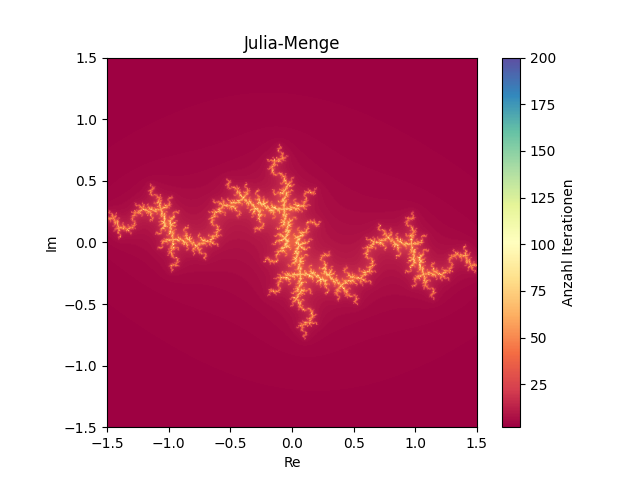
\includegraphics[width=\textwidth]{media/Julia1-spectral.png}
        \caption{Juliamenge für $c=-1+0.3i$}
    \end{subfigure}
    \hfill
    \begin{subfigure}[t]{0.45\textwidth}
        \centering
        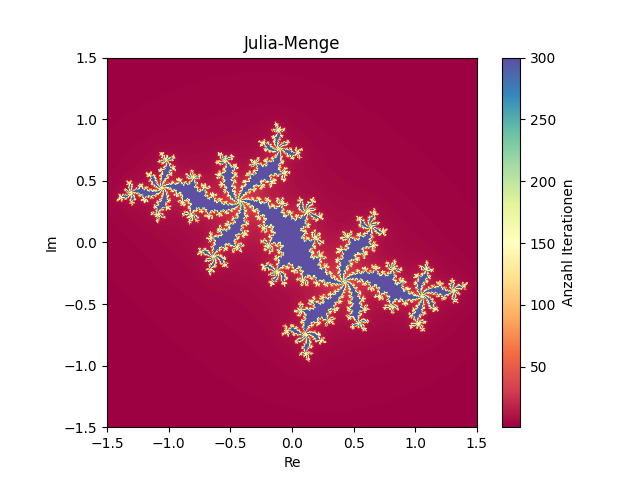
\includegraphics[width=\textwidth]{media/julia2-spectral.png}
        \caption{Juliamenge für $c=-0.5+0.6i$}
    \end{subfigure}
     \begin{subfigure}[t]{0.45\textwidth}
        \centering
        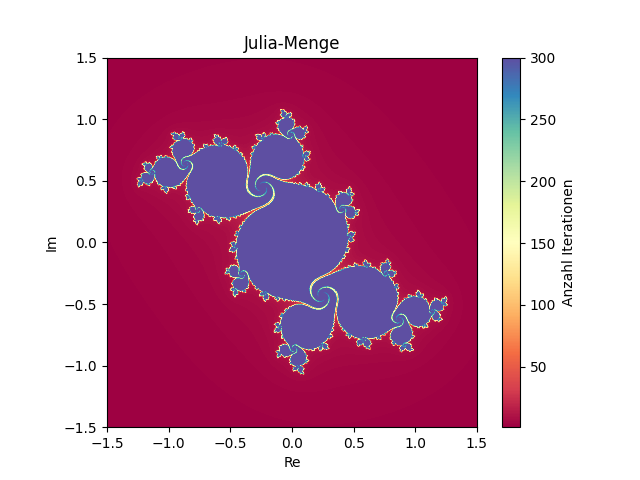
\includegraphics[width=\textwidth]{media/Julia3-spectral.png}
        \caption{Juliamenge für $c=-0.11+0.6557i$}
    \end{subfigure}
    \hfill
    \begin{subfigure}[t]{0.45\textwidth}
        \centering
        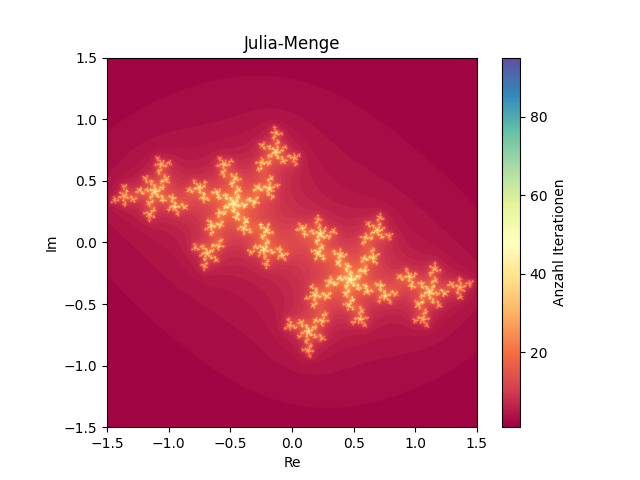
\includegraphics[width=\textwidth]{media/Julia4-spectral.png}
        \caption{Juliamenge für $c=-0.6+0.6i$}
    \end{subfigure}
\end{figure}



\clearpage

Die Bilder oben wurden mit Python erstellt. Das Vorgehen ist grob wie folgt:
\begin{enumerate}
    \item Es wird ein Wert für $c$ in $f(z) = z^2 + c$ festgelegt.
    \item Über einen Bereich der komplexen Zahlenebene (in den Beispielen oben ist es $\RE(z), \IM(z) \in [-1.5, 1.5]$) wird ein feines Gitter gelegt. Jeder Gitterpunkt entspricht dann einem Pixel des Bildes.
    \item Für jeden Gitterpunkt wird die Iteration der Funktion $f$ berechnet. Dabei wird die Anzahl Iterationen bestimmt, die nötig sind, damit der Betrag grösser als eine festgelegte Grenze wird (z. Bsp. 5).
    \item Je nach Anzahl Iterationen wird dem entsprechenden Pixel eine bestimmte Farbe zugeordnet. Damit entsteht eine sogenannte \emph{Heatmap}. Je heller ein Pixel, desto höher ist die Anzahl Iterationen, die nötig waren, damit der Betrag grösser als die Grenze wurde. Je dunkler ein Pixel, desto weniger Iterationen waren nötig.
\end{enumerate}

\begin{LA}
{Heatmaps in Python}{}
Als Erstes müssen Sie sich mit der Bibliothek matplotlib.pyplot vertraut machen. Mit dieser Bibliothek lassen sich Bilder in Python erzeugen.
\begin{enumerate}
    \item Kopieren Sie den folgenden Code und führen Sie ihn aus.
    \lstinputlisting[language=Python]{KomplexeZahlenPython/JuliaMandelbrot/testHeatmap.py}
    \item Verändern Sie das Programm so, dass das Bild eine Art Kreuz darstellt.
\end{enumerate}

Im Folgenden werden Sie einige Optionen des Befehls \lstinline|plt.imshow(bild)| untersuchen.
\begin{enumerate} [resume]
    \item Verändern Sie den Befehl in Zeile 11 wie folgt: \lstinline|plt.imshow(bild,extent=(0, 10, -20, 20))| und beobachten Sie, was passiert.
    \item Der erste Wert \lstinline|bild[0][0]| in der Liste \lstinline|bild| mit dem Wert 1 erscheint in der Grafik ganz oben links. In der Mathematik wird jedoch der Ursprung in der unteren linken Ecke dargestellt. Fügen Sie dem Befehl in Zeile 11 die Option \lstinline|origin='lower'| hinzu, so dass der Befehl wie folgt aussieht: \lstinline|plt.imshow(bild,extent=(0, 10, -20, 20), origin='lower')|. Was passiert nun?
    \item Für die Heatmap gibt es verschiedene Farbskalen. Eine davon ist \lstinline|Spectral|. Fügen Sie dem Befehl in Zeile 11 die Option \lstinline|cmap='Spectral'| hinzu, so dass der Befehl wie folgt aussieht: \lstinline|plt.imshow(bild,extent=(0, 10, -20, 20), origin='lower', cmap='spectral')|. Was passiert nun?
    \item Testen Sie verschiedene Farbskalen. Sie finden Sie in der Dokumentation von \href{https://matplotlib.org/stable/users/explain/colors/colormaps.html}{matplotlib}.
\end{enumerate}

\end{LA}

\begin{LA}
{Programm zur Darstellung der Julia-Menge}{Julia-Menge}
\begin{enumerate}
    \item 
Kopieren Sie das folgende Programm und führen Sie es aus.
\lstinputlisting[language=Python]{KomplexeZahlenPython/JuliaMandelbrot/juliaMenge-V2.py}
\item Diskutieren Sie mit dem*der Banknachbar*in was in den Zeilen 37-46 passiert und beantworten Sie die folgende Frage: Wird das Bild Zeile für Zeile oder Spalte für Spalte aufgebaut?
\item Verändern Sie das Programm so, dass die Julia-Menge für $c = -0.4 + 0.6i$ dargestellt wird.
\item Verändern Sie das Programm so, dass die Julia-Menge der Iteration der Funktion $f(z) = z^3 + c$ berechnet wird.
\end{enumerate}
\end{LA}

\subsubsection*{Mandelbrotmenge}


\begin{definition}
    {Mandelbrotmenge}{}
    Die Mandelbrotmenge ist die Menge aller komplexen Zahlen $c$, für die die Iteration der Funktion $f(z) = z^2 + c$ mit dem Startwert $z_1 = 0$ nicht divergiert.

    Sie wird benannt nach Benoît B. Mandelbrot (1924 - 2010), der sie 1980 entdeckte.
\end{definition}

Mit anderen Worten: Während zur Bestimmung von Juliamengen bei der Funktion $f(z) = z^2 + c$ die Konstante $c$ festgelegt wird und dann die Iteration mit verschiedenen Startwerten $z_1$ untersucht wird, wird bei der Mandelbrotmenge immer mit dem Startwert $z_1 = 0$ gestartet und es werden verschiedene Werte des Parameters $c$ verwendet.

\begin{center}
    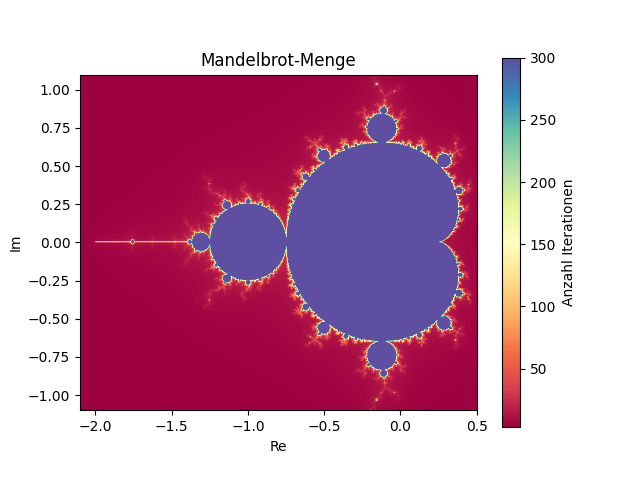
\includegraphics[width = 0.8\textwidth]{media/mandelbrot-spectral.png}
\end{center}

\textbf{Eigenschaften der Mandelbrotmenge $M$:}
\begin{itemize}
    \item $M$ ist ein Fraktal, d. h. es gibt beliebig kleine Ausschnitte von M, welche bei genügender Vergrösserung wieder die Menge M ergeben.
    \item $M$ ist zusammenhängend.
    \item $M$ besteht aus unendlich vielen gleichartigen, selbstähnlichen Teilen. Ein solcher Teil besteht aus einer Herzkurve (Kardioide), an der unendlich viele Kreise angehängt sind. Ferner gehören linienartige Antennen und Fäden zu $M$, welche diese Teile verbinden. Während das Innere der Herzkurve und der Kreise völlig ausgefüllt ist, besteht der Rand aus unbegrenzt vielen, äusserst reichhaltigen Formen.

\end{itemize}
\begin{center}
    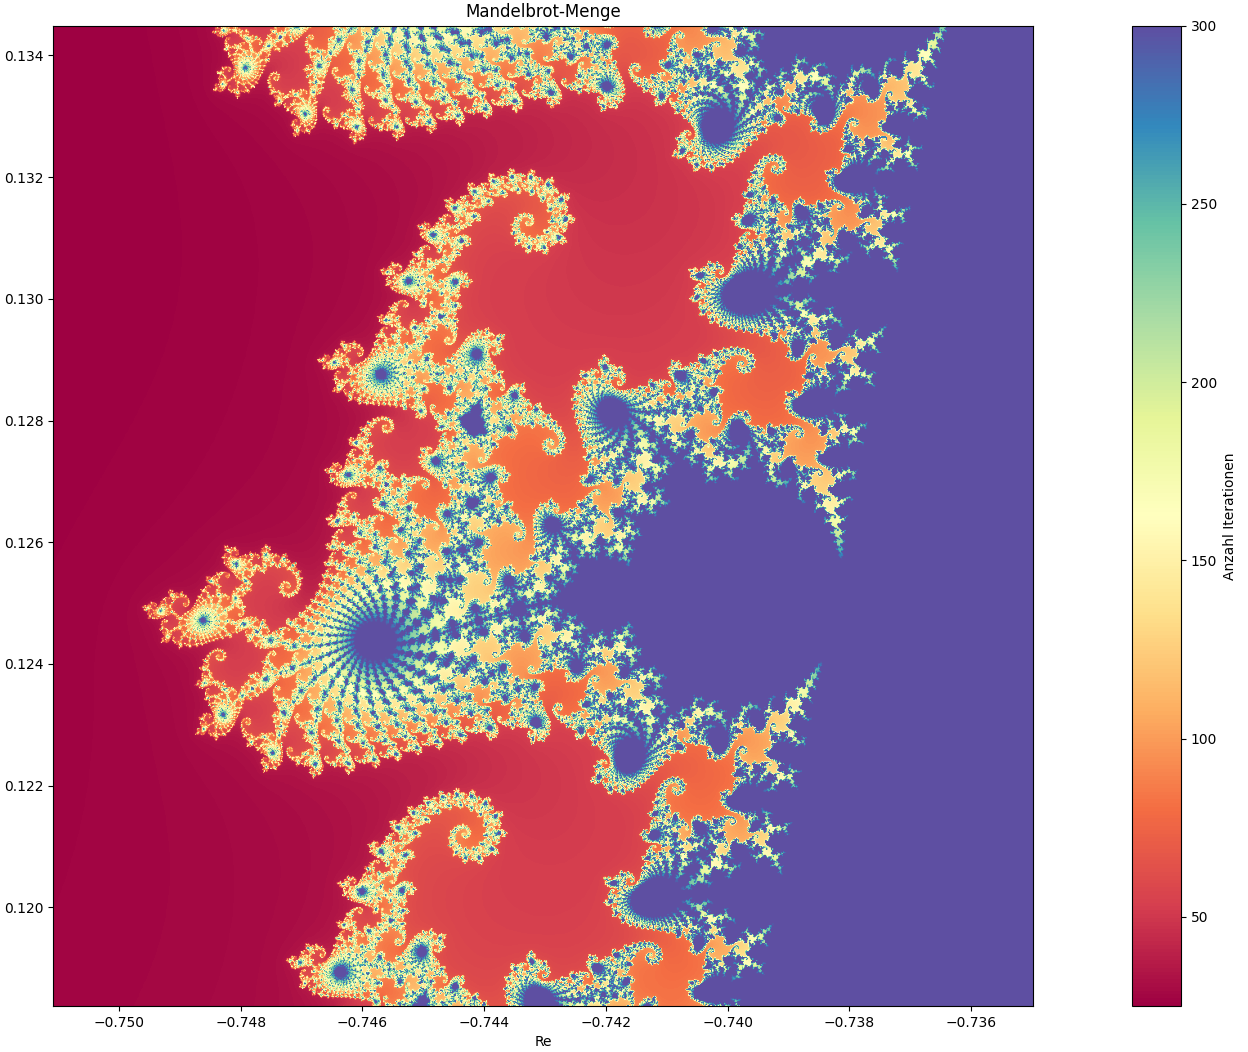
\includegraphics[width = 0.8\textwidth]{media/mandelbrot-zoom3.png}
\end{center}
\begin{ueb}
{Mandelbrotmenge}{}
\begin{enumerate}
    \item Passen Sie das Programm aus der vorherigen \Cref{LA:Julia-Menge} so an, dass die Mandelbrotmenge dargestellt wird. %Verwenden Sie dazu die Funktion $f(z) = z^2 + c$ mit dem Startwert $z_1 = 0$ und variieren Sie den Wert von $c$.
    \item Zoomen Sie in die Mandelbrotmenge hinein, indem Sie den Bereich der komplexen Zahlenebene, der dargestellt wird, verkleinern. Versuchen Sie z.B. den Bereich $\RE(c) = -0.743 566 9 \pm 0.00115$ und $\IM(c) =  0.131 402 3 \pm 0.00115$ darzustellen.

    Je nach Rechenleistung Ihres Computers können Sie die Auflösung des Bildes verändern.
    \item Suchen Sie im Internet nach Video mit den Stichwörtern \emph{Mandelbrot} und \emph{Zoom} und staunen Sie.
\end{enumerate}

\end{ueb}
%\input{todo.tex}


	
\end{document}